\documentclass[a4paper,12pt]{report}

% ── Paquetes ─────────────────────────────────────────────────────────────────
\usepackage[utf8]{inputenc}
\usepackage[spanish]{babel}
\usepackage{geometry}
\usepackage{graphicx}
\usepackage{hyperref}
\usepackage{xcolor}
\usepackage{float}
\usepackage{booktabs}
\usepackage{longtable}
\usepackage{array}
\usepackage{listings}
\usepackage{caption}
\usepackage{subcaption}
\usepackage{parskip}
\usepackage{setspace}
\usepackage{fancyhdr}
\usepackage{titlesec}
\usepackage{enumitem}
\usepackage{tabularx}
\usepackage{multirow}
\usepackage[most]{tcolorbox}
\usepackage{tabularx}
% \usepackage{tikz}  % descomentar si se añaden diagramas TikZ

% ── Profundidad del índice ───────────────────────────────────────────────────
% Se muestran capítulos y secciones para que el índice mantenga una estructura clara.
\setcounter{tocdepth}{1}
\setcounter{secnumdepth}{3}

% ── Configuración de márgenes ────────────────────────────────────────────────
\geometry{left=2.5cm, right=2.5cm, top=2.5cm, bottom=2.5cm}
\setlength{\headheight}{14pt}

% ── Interlineado ─────────────────────────────────────────────────────────────
\setstretch{1.15}

% ── Colores ──────────────────────────────────────────────────────────────────
\definecolor{codeblue}{RGB}{46, 117, 182}
\definecolor{codegray}{RGB}{245, 245, 245}
\definecolor{codered}{RGB}{192, 0, 0}

% ── Configuración de listings ────────────────────────────────────────────────
\lstset{
  backgroundcolor=\color{codegray},
  basicstyle=\ttfamily\small,
  breakatwhitespace=false,
  breaklines=true,
  captionpos=b,
  frame=single,
  rulecolor=\color{gray!40},
  showstringspaces=false,
  tabsize=2,
  numbers=left,
  numberstyle=\tiny\color{gray},
  xleftmargin=1.5em,
  framexleftmargin=1.5em
}

% ── Configuración de hyperref ────────────────────────────────────────────────
\hypersetup{
  colorlinks=false,
  linkbordercolor=white,
  urlbordercolor=white,
  citebordercolor=white,
  pdftitle={OmniLitter — Sistema multiplataforma para la gestión y análisis de datos de contaminación por residuos},
  pdfauthor={Alejandro Castilla, Ignacio Martínez Díaz}
}

% ── Cabecera y pie de página ─────────────────────────────────────────────────
\pagestyle{fancy}
\fancyhf{}
\fancyhead[L]{\small OmniLitter — Monitorización de residuos}
\fancyhead[R]{\small Universidad de Sevilla}
\fancyfoot[C]{\thepage}
\renewcommand{\headrulewidth}{0.4pt}

% ── Formato de títulos ───────────────────────────────────────────────────────
\titleformat{\chapter}
  {\huge\bfseries}
  {\thechapter.}{0.8em}{}

\titleformat{\section}
  {\large\bfseries}
  {\thesection.}{0.5em}{}[\titlerule]

\titleformat{\subsection}
  {\normalsize\bfseries}
  {\thesubsection.}{0.5em}{}

\titleformat{\subsubsection}
  {\normalsize\bfseries}
  {\thesubsubsection.}{0.5em}{}

% ── Captions de tablas y figuras ─────────────────────────────────────────────
\captionsetup[table]{labelfont=bf, position=above}
\captionsetup[figure]{labelfont=bf, position=below}

% ═════════════════════════════════════════════════════════════════════════════
\begin{document}

% ── PORTADA ──────────────────────────────────────────────────────────────────
\begin{titlepage}
  \centering
  \vspace*{1cm}
  
  {\LARGE \textbf{OmniLitter} \par}
  \vspace{0.4cm}  
  {\Large Sistema multiplataforma para la gestión y análisis de datos de contaminación por residuos \par}

  \vspace{2.5cm}

  
\includegraphics[width=0.72\textwidth]{figures/logo-ETSII-US-Vertical-Negro.png} \par

  \vfill

  \begin{minipage}{0.9\textwidth}

    {\large \textbf{Trabajo Fin de Grado} \par}
    \vspace{0.2cm}
    {\large \textbf{Grado:} Ingeniería Informática - Ingeniería del Software \par}
    \vspace{0.2cm}
    {\large \textbf{Centro:} ETSII — Universidad de Sevilla \par}
    \vspace{0.2cm}
    {\large \textbf{Curso académico:} 2025/26 \par}
    \vspace{0.5cm}

    \textbf{Autores:} \par
    \vspace{0.1cm}
    \begin{itemize}[leftmargin=1.5em]
      \item Alejandro Castilla — alecasbar@alum.us.es
      \item Ignacio Martínez Díaz — ignmardia1@alum.us.es
    \end{itemize}

    \vspace{0.3cm}
    {\large \textbf{Tutor académico:} Cruz Mata, Fermín \par}
    \vspace{0.2cm}
    {\large \textbf{Cotutor:} Ortega Rodríguez, Francisco Javier \par}
    \vspace{0.2cm}
    {\large \textbf{Cliente / entidad colaboradora:} Daniel González Fernández / Universidad de Cádiz \par}

    % Opcional:
    % \vspace{0.3cm}
    % {\large \textbf{Repositorio:} \href{URL}{\texttt{URL}} \par}

  \end{minipage}

\end{titlepage}

% ── ÍNDICES ──────────────────────────────────────────────────────────────────
\pagenumbering{roman}
\pagestyle{plain}

\chapter*{Resumen}
\clearpage

\chapter*{Abstract}
\clearpage

\tableofcontents
\clearpage

\listoffigures
\clearpage

\listoftables
\clearpage

\pagenumbering{arabic}
\pagestyle{fancy}

% ── CAPÍTULOS PRINCIPALES ────────────────────────────────────────────────────
\chapter{Introducción}

\section{Contexto y motivación}

La contaminación por residuos en entornos terrestres y acuáticos constituye uno de
los principales problemas ambientales actuales. La presencia de basura en ríos,
playas, zonas costeras, bosques, áreas urbanas y otros espacios naturales afecta
a los ecosistemas, a la biodiversidad y a la calidad de vida de las personas.
Para comprender la magnitud del problema y evaluar la eficacia de las medidas de
prevención o mitigación, las administraciones públicas, las instituciones
científicas y las organizaciones ambientales impulsan programas de monitorización
de residuos en distintos compartimentos ambientales.

La utilidad de estos programas depende de que los datos recogidos sean
comparables, estén correctamente georreferenciados y conserven información
suficiente sobre cómo, cuándo y dónde se han obtenido. En el caso de las basuras
fluviales, el Joint Research Centre de la Comisión Europea señala la falta de
información sistemática sobre la cantidad de residuos transportados por los ríos
y la ausencia de metodologías armonizadas capaces de generar datos cuantitativos
comparables \cite{gonzalez2016riverine}. De forma similar, trabajos recientes
subrayan la necesidad de armonizar las técnicas de monitorización de
macroplásticos en ecosistemas acuáticos y terrestres
\cite{gallitelli2024macroplastics}.

Un antecedente directo de este proyecto es el trabajo realizado para la
monitorización de macrobasuras flotantes en ríos, donde se desarrolló una
aplicación para dispositivos tipo \textit{tablet} capaz de registrar los ítems
observados, su tamaño y su posición geográfica durante sesiones de
monitorización \cite{gonzalezfernandez2017harmonized}. Este antecedente refuerza
la idea de que la herramienta de captura no debe limitarse a digitalizar un
formulario, sino que debe orientar la observación y conservar desde el inicio los
datos necesarios para que los registros puedan compararse posteriormente.

En este contexto, el cliente planteó la necesidad de renovar y ampliar la
aplicación \textit{Floating Litter Monitoring}. La herramienta original estaba
orientada principalmente a la monitorización de residuos en ríos y mares,
mientras que el nuevo proyecto debía extender esa capacidad a una mayor variedad
de entornos naturales y urbanos, incorporar una gestión más flexible de usuarios
y grupos, mejorar la recogida de evidencias y permitir la consulta posterior de
los datos desde un portal web.

Como respuesta a esta necesidad se propone el desarrollo de OmniLitter, una
plataforma formada por una aplicación móvil, un portal web y un backend
centralizado. Su finalidad es facilitar la recogida, gestión y análisis de datos
de residuos mediante una solución que combine trabajo de campo, sincronización de
información, control de permisos y explotación posterior de los datos
recopilados.

\section{Problema abordado}

La monitorización de residuos requiere la participación de distintas personas y
grupos que realizan campañas en lugares y momentos diferentes. Si la información
se registra mediante formularios no normalizados, hojas de cálculo aisladas o
campañas de limpieza sin un protocolo común, los datos resultantes suelen quedar
dispersos, son difíciles de comparar y pierden parte de su valor para análisis
científicos posteriores.

Además, la captura de datos se realiza habitualmente en la naturaleza, donde la
conectividad a Internet puede ser limitada o inexistente. Esta situación dificulta
el uso de soluciones que dependen de una conexión permanente con servidores
remotos. Por ello, resulta necesario que la aplicación móvil pueda almacenar
sesiones, observaciones, fotografías y metadatos en el propio dispositivo, y que
sincronice esa información con el servidor cuando vuelva a existir conexión.

El proyecto también exige registrar datos con suficiente calidad científica. Cada
observación debe asociarse a una taxonomía de residuos, una localización
geográfica, una fecha y hora, evidencias fotográficas y metadatos de muestreo
como el entorno, la tipología, el método empleado, la duración, el transecto o el
área observada. La precisión de la posición GPS y el estado de sincronización de
cada registro también son relevantes para interpretar correctamente los datos
recogidos.

A estas necesidades se suma la organización colaborativa del trabajo. Los
usuarios pertenecen a grupos, los grupos gestionan campañas, las campañas
contienen sesiones de muestreo y las sesiones agrupan observaciones. Esta
estructura requiere mecanismos de autenticación, control de permisos y aislamiento
de datos para que cada equipo pueda gestionar su información de forma segura y
privada.

Por tanto, el problema abordado no consiste únicamente en crear un formulario
digital de recogida de residuos. El reto es diseñar una plataforma que conecte la
captura offline en campo con una infraestructura común de almacenamiento,
administración, visualización y exportación, manteniendo la trazabilidad y la
comparabilidad de los datos desde su origen.

\section{Objetivos}

El objetivo principal de este Trabajo Fin de Grado es diseñar, desarrollar e
implementar OmniLitter, una plataforma software multiplataforma que facilite la
monitorización de residuos en distintos entornos naturales y permita transformar
observaciones de campo en datos estructurados, comparables y reutilizables.

Para alcanzar este objetivo general se establecen los siguientes objetivos
específicos:

\begin{enumerate}
    \item Diseñar una arquitectura software que integre una aplicación móvil, un
    portal web, un backend centralizado y una base de datos común.

    \item Organizar la información del sistema mediante grupos de trabajo,
    campañas, sesiones de muestreo y observaciones geolocalizadas.

    \item Desarrollar una aplicación móvil destinada a la captura de datos en
    campo, incluyendo residuos observados, fotografías, ubicación, fecha, hora y
    metadatos de muestreo.

    \item Permitir el funcionamiento de la aplicación móvil en condiciones de
    conectividad limitada mediante persistencia local y sincronización diferida
    con el servidor.

    \item Incorporar taxonomías estandarizadas, entornos, tipologías y métodos
    de muestreo configurables para favorecer la calidad científica de la
    información registrada.

    \item Implementar mecanismos de autenticación, roles, permisos y aislamiento
    de datos entre grupos de trabajo.

    \item Desarrollar un portal web que facilite la administración de usuarios,
    grupos y campañas, así como la consulta de sesiones y observaciones
    recopiladas.

    \item Proporcionar herramientas de visualización y explotación de datos,
    incluyendo mapas, paneles informativos y exportación en formatos adecuados
    para análisis posterior.

    \item Garantizar la integridad, trazabilidad y consistencia de la información
    almacenada mediante un backend centralizado y una API autenticada.

    \item Aplicar metodologías y herramientas de ingeniería del software para
    documentar, probar y validar la solución desarrollada dentro del alcance
    académico del proyecto.
\end{enumerate}

\section{Alcance del proyecto}

El presente Trabajo Fin de Grado aborda el diseño, desarrollo e implementación de
una versión funcional de una plataforma software denominada OmniLitter, orientada
a facilitar la monitorización y el análisis de la contaminación por residuos en
distintos ecosistemas terrestres, acuáticos y urbanos, dentro del alcance
académico del proyecto.

La solución desarrollada está compuesta por una aplicación móvil destinada a la
recogida de información en campo, un portal web para la gestión y explotación de
los datos recopilados, y un backend centralizado encargado de la autenticación,
la lógica de negocio, la sincronización y la persistencia de la información.

Dentro del alcance del proyecto se incluyen las siguientes funcionalidades:

\begin{itemize}
    \item Diseño e implementación de la arquitectura completa del sistema,
    incluyendo aplicación móvil, portal web, backend y base de datos.

    \item Registro de observaciones de residuos utilizando una taxonomía
    jerárquica estandarizada que garantice la consistencia científica de los
    datos.

    \item Captura automática de información geográfica y temporal asociada a cada
    observación mediante los sensores disponibles en los dispositivos móviles.

    \item Gestión de fotografías y metadatos asociados a las observaciones
    registradas.

    \item Gestión de campañas y sesiones de muestreo, incluyendo información
    contextual como el entorno analizado, el método empleado, la duración de la
    sesión, el tipo de transecto o cuadrante y las características del área
    estudiada.

    \item Funcionamiento en modo offline mediante almacenamiento local de la
    información y sincronización posterior con el servidor cuando exista
    conectividad.

    \item Administración de campañas, usuarios, grupos y permisos mediante un
    portal web de gestión.

    \item Visualización de observaciones, sesiones y campañas mediante mapas
    interactivos y paneles informativos.

    \item Exportación de los datos recopilados en formatos adecuados para su
    posterior explotación y análisis científico.

    \item Implementación de mecanismos de autenticación, control de acceso y
    protección de la información almacenada.

    \item Elaboración de la documentación técnica, manuales, pruebas y memoria
    académica asociada al desarrollo del sistema.
\end{itemize}

Quedan fuera del alcance del Trabajo Fin de Grado el mantenimiento
post-producción, el soporte técnico continuo tras la entrega y la definición de
nuevos protocolos científicos oficiales. De esta forma, el alcance del proyecto
se centra en proporcionar una plataforma funcional para la recogida, gestión,
consulta y explotación de datos relacionados con la monitorización de residuos,
estableciendo una base tecnológica que permita futuras ampliaciones y desarrollos.
\newpage

\chapter{Contexto y antecedentes}

\section{Monitorización de residuos}

\section{Aplicaciones de campo y ciencia ciudadana}

\section{Herramientas existentes}

\section{Taxonomías y datos científicos}

\section{Conclusiones del análisis}

\newpage

\chapter{Descripción del proyecto}

\section{Visión general de OmniLitter}

OmniLitter es una plataforma multiplataforma desarrollada con el objetivo de facilitar la monitorización y el análisis de residuos en distintos tipos de entornos: playas, riberas, bosques y zonas urbanas. El sistema está orientado tanto a investigadores como a colaboradores de campo, proporcionando herramientas que permiten registrar, almacenar y analizar información relacionada con campañas de muestreo de residuos.

La finalidad de la plataforma no es únicamente contabilizar residuos, sino digitalizar y unificar la toma de datos para que las observaciones puedan convertirse en información científica comparable. Para ello, OmniLitter organiza el trabajo en campañas y sesiones de muestreo, registra metadatos de campo, utiliza categorías estandarizadas de residuos y conserva la localización y evidencias asociadas a cada observación.

La arquitectura de OmniLitter se compone de tres elementos principales estrechamente
integrados: una API central, una aplicación móvil y un portal web. La aplicación
móvil se orienta a la recogida de datos en campo, el portal web a la gestión y
explotación de la información, y la API actúa como punto común de autenticación,
validación, persistencia y sincronización.

Esta aproximación permite conectar la recogida de datos con la evaluación de tendencias y medidas de mitigación. Al conservar datos cuantitativos, metadatos y trazabilidad por campaña, la plataforma puede apoyar comparaciones antes y después de una intervención, ayudar a identificar fuentes probables de contaminación y aportar evidencias para valorar la eficacia de políticas o acciones de reducción de residuos.

\section{Actores y perfiles de usuario}

OmniLitter es una plataforma colaborativa en la que distintos usuarios participan en la gestión de campañas de monitorización y en la recogida de observaciones de residuos. Debido a esta naturaleza colaborativa, el sistema implementa un modelo de control de acceso basado en dos conceptos diferenciados: el rol global del usuario dentro de la plataforma y el rol que dicho usuario posee dentro de cada grupo de trabajo.

Esta separación permite que una misma persona pueda desempeñar diferentes responsabilidades según el grupo en el que participe, garantizando al mismo tiempo el aislamiento de la información entre equipos de trabajo independientes.

El acceso a los datos se estructura alrededor de tres elementos fundamentales:

\begin{itemize}
    \item La cuenta de usuario, que identifica a la persona dentro de la plataforma.
    \item El grupo de trabajo, que delimita el conjunto de campañas, sesiones y observaciones accesibles.
    \item El rol asignado, que determina las acciones que el usuario puede realizar sobre dichos datos.
\end{itemize}

\begin{figure}[H]
\centering
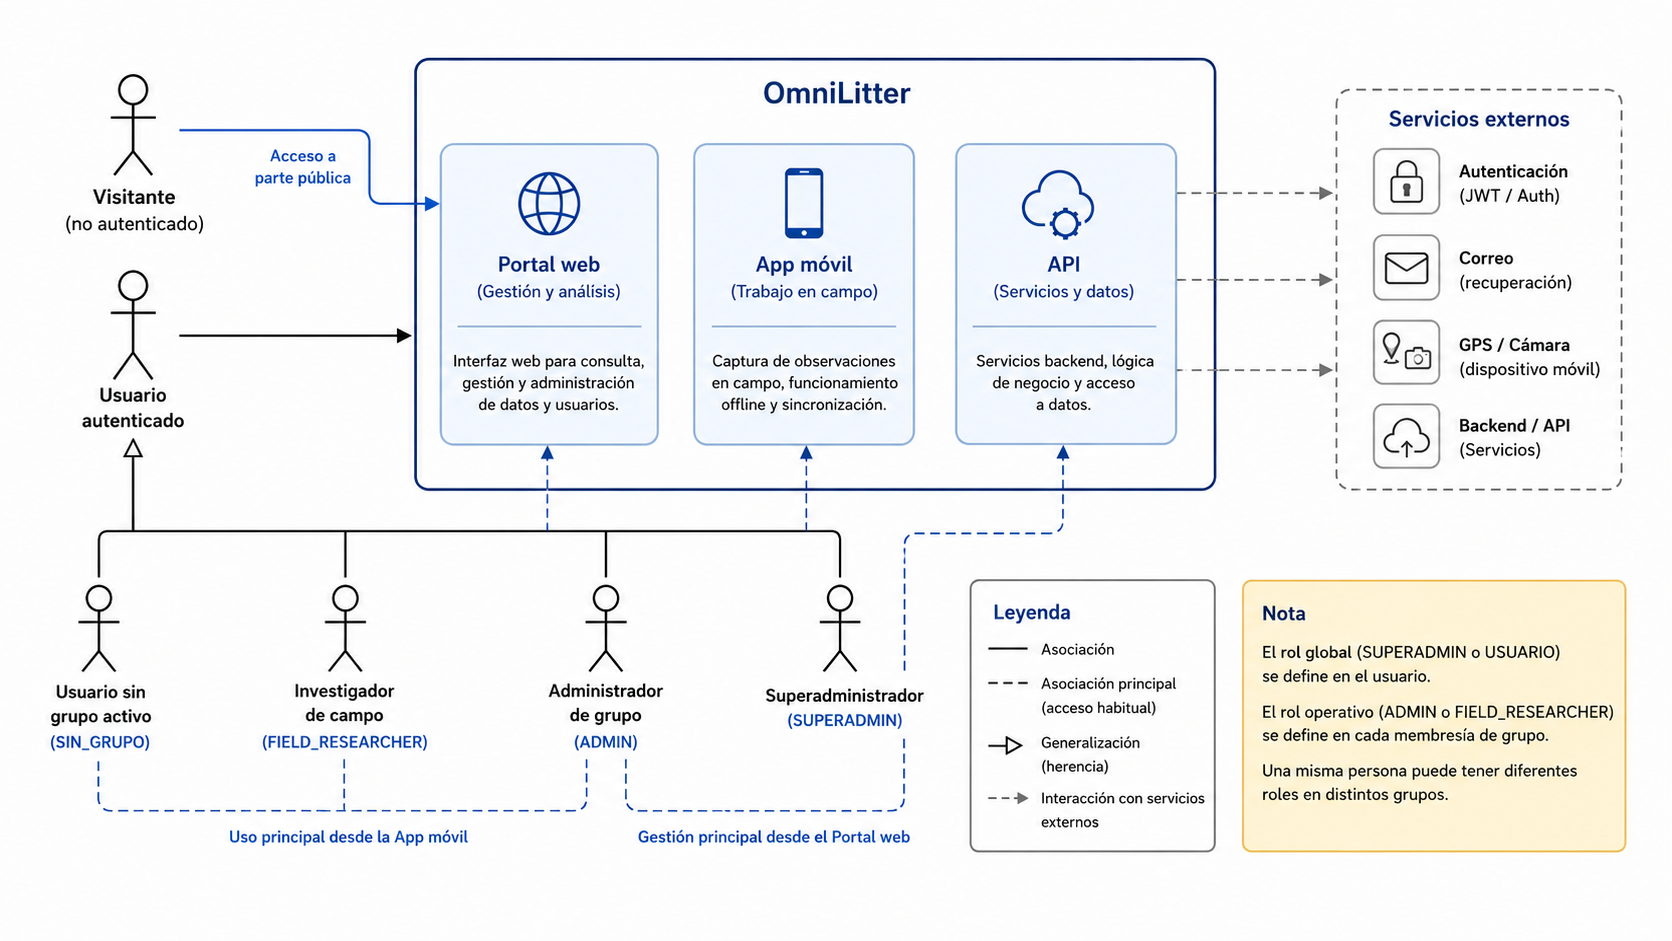
\includegraphics[width=0.92\textwidth]{figures/actores_perfiles.png}
\caption{Actores y perfiles de usuario contemplados en OmniLitter.}
\label{fig:actores_perfiles}
\end{figure}

A continuación se describen los principales perfiles contemplados por el sistema.

\subsection{Visitante}

El visitante corresponde a cualquier persona que accede a la parte pública de la plataforma sin haber iniciado sesión. Este perfil únicamente puede consultar información general sobre OmniLitter y acceder a las funcionalidades de autenticación, como el inicio de sesión, el registro de una nueva cuenta o la recuperación de contraseña.

No dispone de acceso a campañas, observaciones, métricas ni información perteneciente a los grupos de trabajo.

\subsection{Usuario autenticado}

El usuario autenticado constituye el perfil base del sistema. Se trata de cualquier persona que dispone de una cuenta válida y ha iniciado sesión correctamente.

Este perfil puede gestionar la información asociada a su propia cuenta, consultar los grupos a los que pertenece, seleccionar un grupo activo y aceptar o rechazar invitaciones recibidas. Sin embargo, los permisos operativos sobre campañas y observaciones dependen del rol que posea dentro de cada grupo.

\subsection{Investigador de campo}

El investigador de campo es el perfil responsable de la recogida de información durante las campañas de monitorización. Su actividad principal se desarrolla mediante la aplicación móvil, desde la cual puede crear sesiones de muestreo, registrar observaciones, clasificar residuos mediante la taxonomía disponible, adjuntar fotografías y capturar la localización geográfica de cada registro.

Además, este perfil puede trabajar en modo offline cuando no existe conectividad, almacenando localmente la información para sincronizarla posteriormente con el servidor.

Aunque puede consultar la información necesaria para desarrollar su trabajo, no dispone de permisos para administrar usuarios, gestionar campañas o modificar la estructura organizativa del grupo.

\subsection{Administrador de grupo}

El administrador de grupo es el responsable de coordinar la actividad de un grupo de trabajo concreto. Este perfil puede gestionar los miembros del grupo, enviar invitaciones, asignar roles de membresía y administrar las campañas asociadas a dicho grupo.

Entre sus funciones se encuentran la creación, edición y organización de campañas de monitorización, así como la supervisión de la actividad realizada por los investigadores de campo. También dispone de acceso a métricas agregadas e información de seguimiento relacionada con las campañas del grupo.

Sus permisos se limitan exclusivamente a los grupos en los que posee dicho rol. Por tanto, un mismo usuario puede actuar como administrador en un grupo y como investigador de campo en otro diferente.

\subsection{Superadministrador}

El superadministrador representa el perfil con mayor nivel de autoridad dentro de OmniLitter. Su función principal consiste en administrar la plataforma a nivel global y garantizar su correcto funcionamiento.

Este perfil puede gestionar usuarios, modificar roles globales, supervisar grupos de trabajo y realizar tareas de soporte operativo dentro de la plataforma. A diferencia del administrador de grupo, sus permisos no se encuentran restringidos a un único grupo, sino que abarcan la totalidad del sistema.

Debido a su alcance, este perfil está destinado a tareas de administración y soporte de la plataforma, y no a la realización de actividades habituales de monitorización en campo.

\subsection{Usuario sin grupo activo}

Finalmente, OmniLitter contempla la situación de usuarios registrados que todavía no pertenecen a ningún grupo o que no han seleccionado uno como grupo activo.

En este estado, el usuario puede gestionar su cuenta personal y revisar invitaciones pendientes, pero no tiene acceso a campañas, observaciones ni funcionalidades relacionadas con la monitorización hasta incorporarse a un grupo de trabajo.

\subsection{Actores de apoyo}

Además de los usuarios que interactúan directamente con la plataforma, OmniLitter depende de diversos componentes técnicos que permiten el funcionamiento del sistema.

Entre ellos destacan el servicio de autenticación encargado de validar credenciales y gestionar sesiones, el servicio de correo utilizado para determinadas comunicaciones automáticas, los dispositivos móviles empleados durante las campañas de campo y la infraestructura backend responsable de la lógica de negocio y el almacenamiento persistente de la información.

Aunque estos elementos no representan usuarios propiamente dichos, constituyen actores fundamentales para la correcta ejecución de los procesos definidos por la plataforma.

\section{Plataformas del sistema}

OmniLitter se concibe como una plataforma compuesta por varios elementos que colaboran entre sí para cubrir las distintas fases del proceso de monitorización de residuos. La naturaleza del problema exige disponer de herramientas adaptadas tanto al trabajo de campo como a la gestión y análisis posterior de la información recopilada.

Para dar respuesta a estas necesidades, el sistema se estructura en tres componentes principales: una aplicación móvil, un portal web y un backend centralizado. Esta separación permite adaptar cada componente a las tareas específicas que debe desempeñar, manteniendo al mismo tiempo una gestión unificada de la información.

\begin{figure}[H]
\centering
\begin{subfigure}{0.86\textwidth}
    \centering
    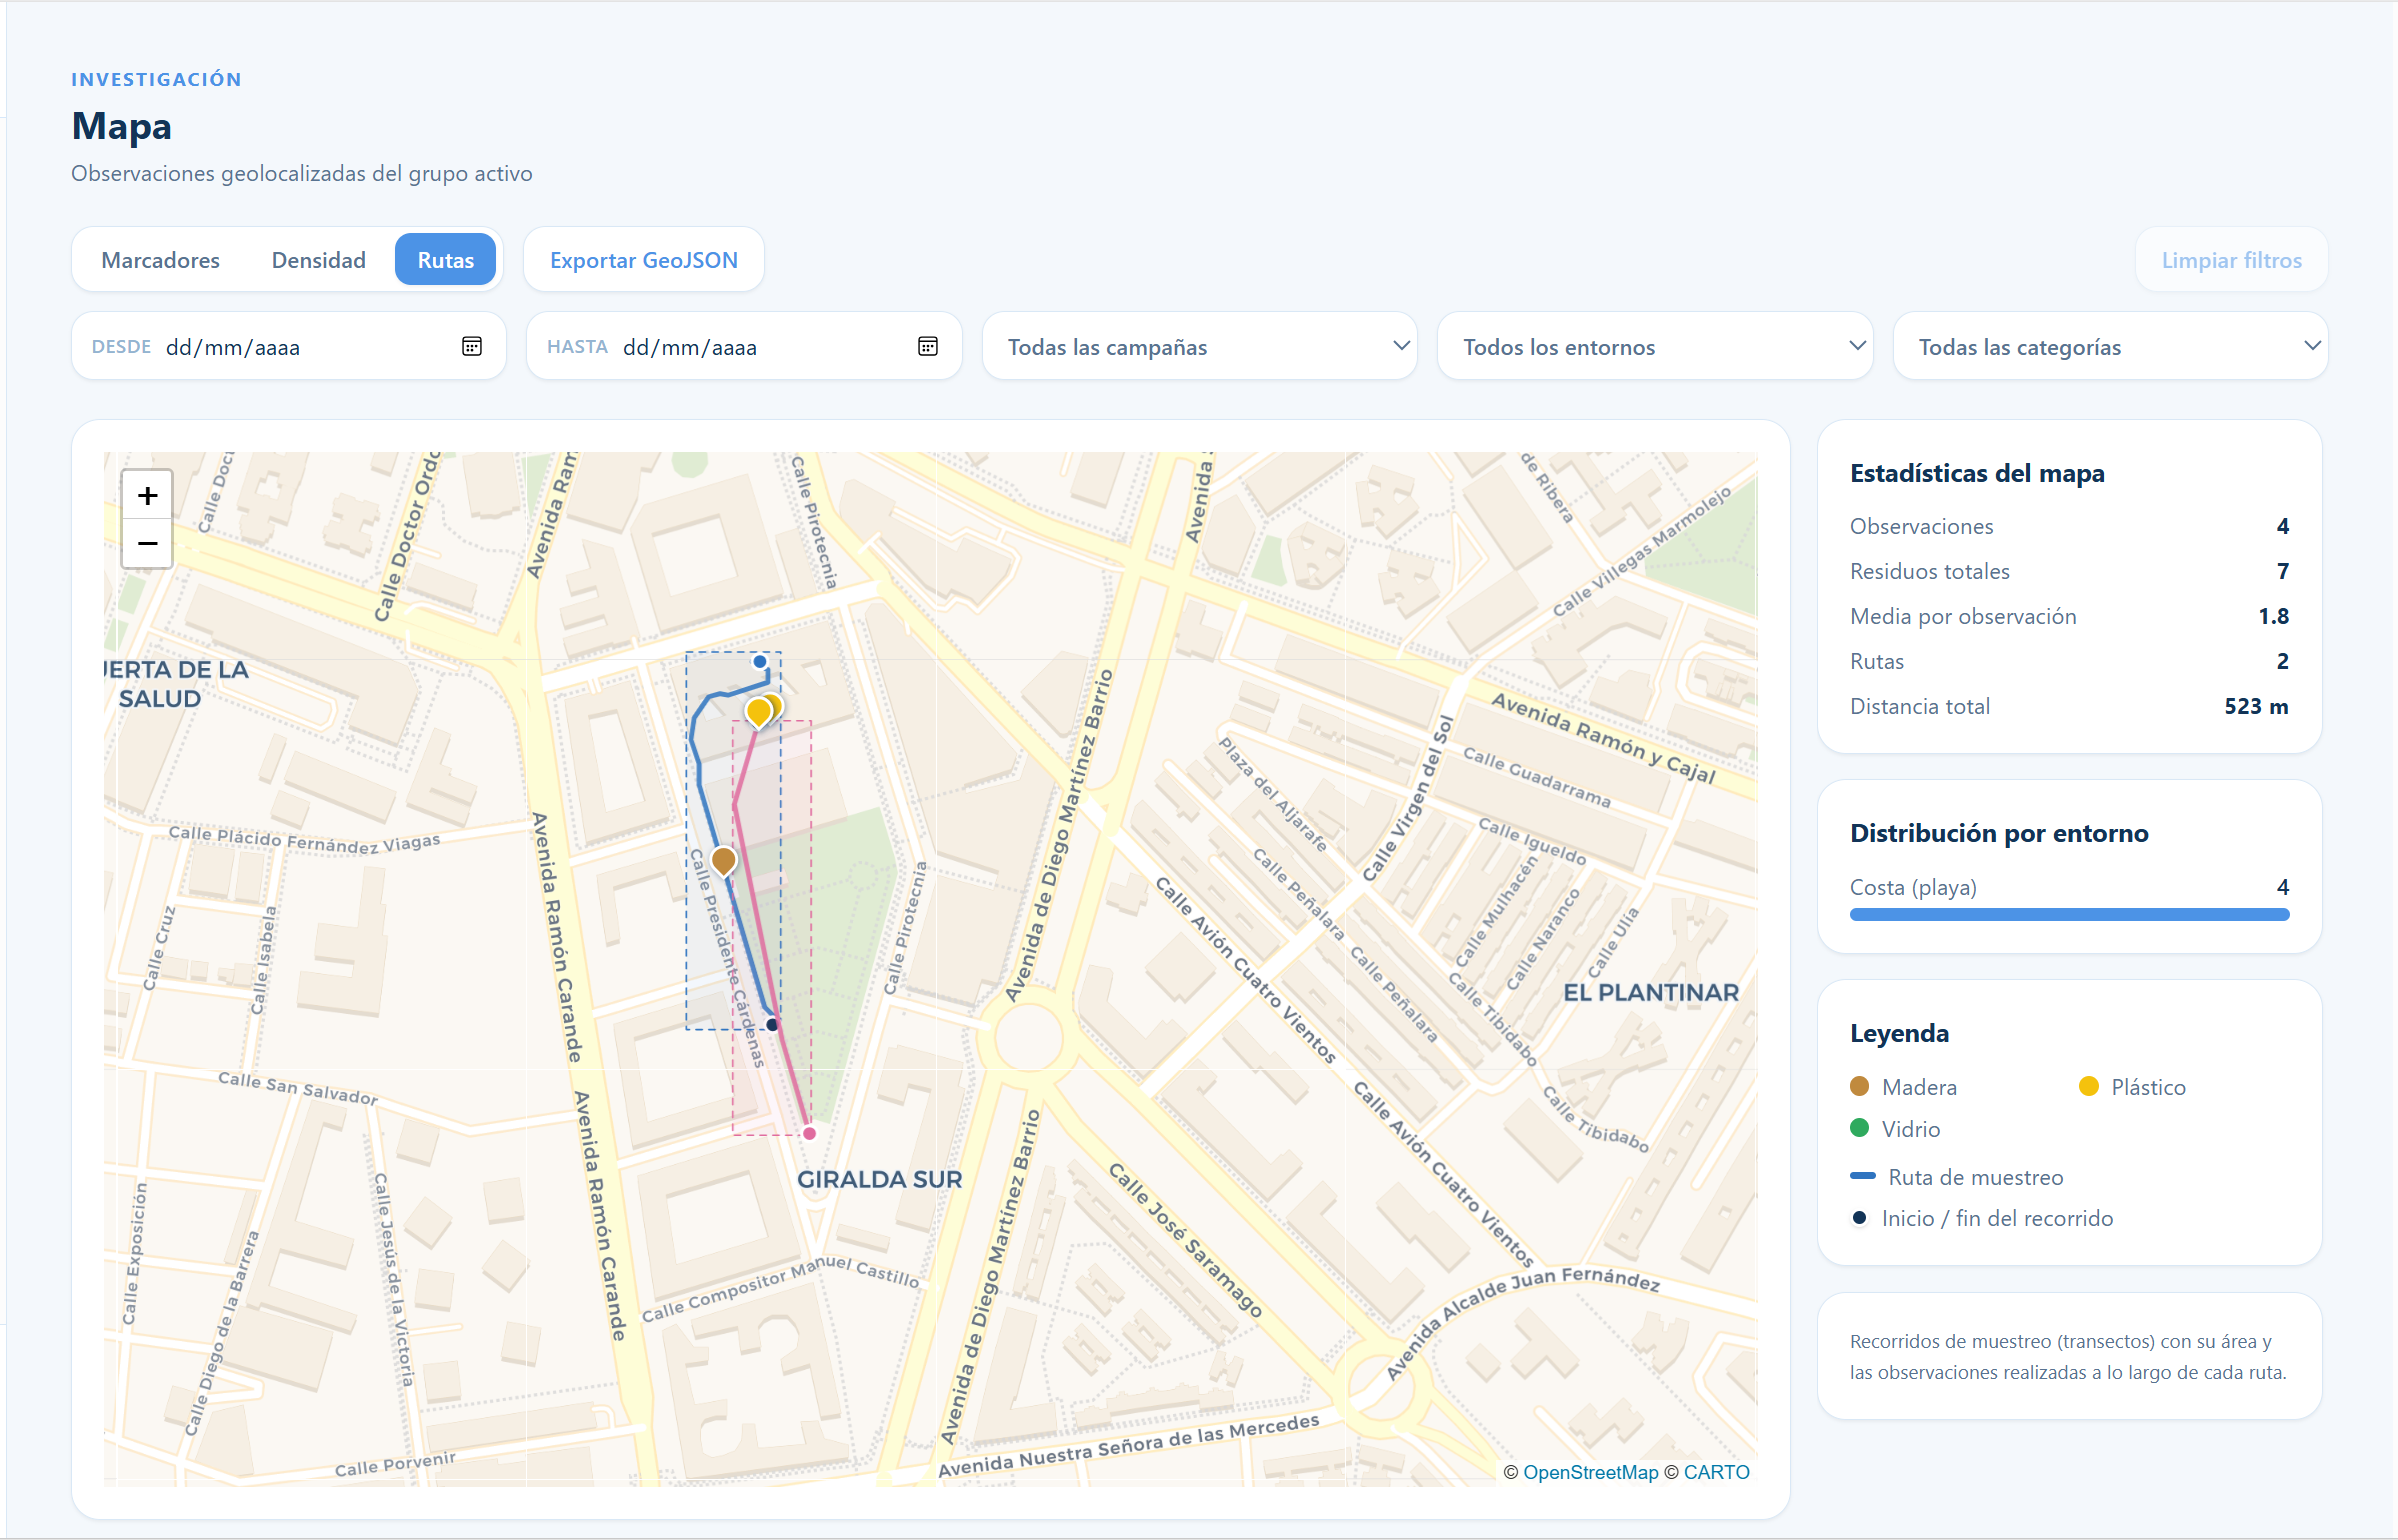
\includegraphics[width=\textwidth]{figures/mapa-web.png}
    \caption{Portal web para la consulta geográfica de observaciones.}
\end{subfigure}

\vspace{0.45em}

\begin{subfigure}{0.30\textwidth}
    \centering
    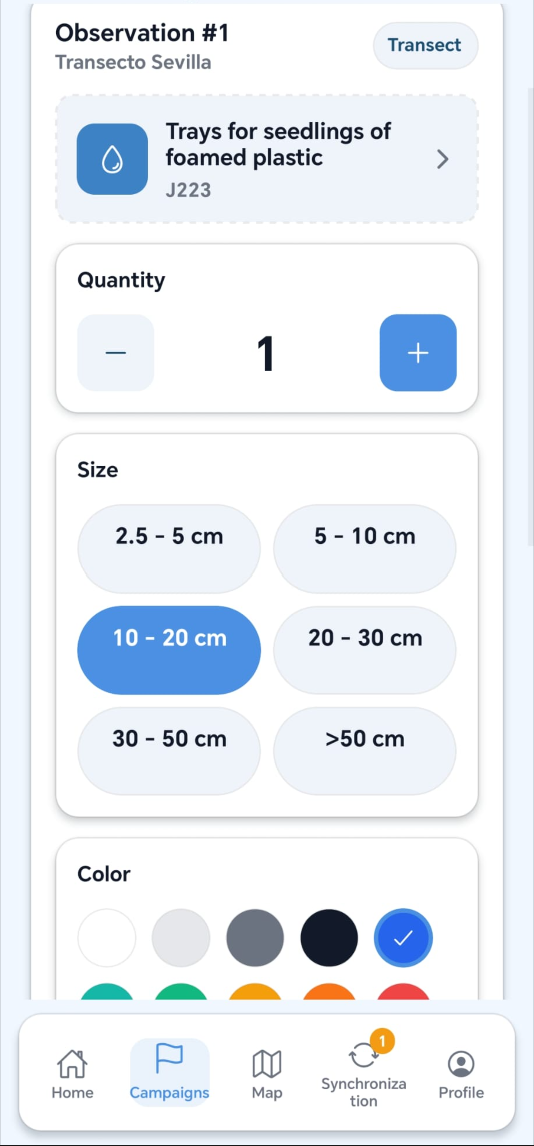
\includegraphics[width=\textwidth]{figures/creacion-observacion-movil.png}
    \caption{Aplicación móvil para el registro de observaciones en campo.}
\end{subfigure}
\caption{Vista general de las dos plataformas principales utilizadas por OmniLitter.}
\label{fig:vista_producto_web_movil}
\end{figure}

\subsection{Aplicación móvil}

La aplicación móvil constituye la herramienta principal para la recogida de datos en campo. Está orientada a los usuarios que participan directamente en las campañas de monitorización y les permite registrar observaciones de residuos en el lugar donde se producen.

A través de esta aplicación es posible consultar campañas, iniciar sesiones de muestreo, registrar observaciones, capturar fotografías asociadas a los residuos encontrados y almacenar la localización geográfica de cada registro. Además, la aplicación está diseñada para funcionar en entornos con conectividad limitada, permitiendo continuar el trabajo incluso cuando no existe acceso a Internet y sincronizando posteriormente la información con el servidor.

\subsection{Portal web}

El portal web proporciona las herramientas necesarias para la gestión y supervisión de la información recopilada. Esta plataforma está orientada principalmente a administradores de grupo, investigadores y superadministradores.

Desde el portal web es posible gestionar usuarios y grupos de trabajo, crear y administrar campañas de monitorización, consultar observaciones registradas, visualizar información geográfica mediante mapas interactivos y acceder a métricas agregadas sobre los datos recopilados. Asimismo, permite exportar la información para su utilización en procesos posteriores de análisis científico.

A diferencia de la aplicación móvil, cuyo objetivo principal es facilitar la recogida de datos en campo, el portal web está enfocado a la coordinación, revisión y explotación de la información almacenada.

\subsection{Backend y almacenamiento centralizado}

El backend actúa como elemento de coordinación entre las distintas plataformas del sistema. Su función consiste en centralizar la lógica de negocio, gestionar la autenticación de usuarios, controlar los permisos de acceso y garantizar la consistencia de los datos almacenados.

Tanto la aplicación móvil como el portal web se comunican con este componente para consultar o registrar información. De esta forma, todas las operaciones se realizan sobre una única fuente de datos común, evitando inconsistencias y facilitando la gestión centralizada del sistema.

La información recopilada durante las campañas se almacena en una base de datos centralizada que actúa como repositorio principal de usuarios, grupos, campañas, sesiones de muestreo, observaciones y fotografías asociadas.

\subsection{Integración de las plataformas}

La combinación de estas plataformas permite cubrir el ciclo completo de trabajo de una campaña de monitorización. La aplicación móvil facilita la recogida de datos sobre el terreno, el backend garantiza la gestión y consistencia de la información, y el portal web proporciona las herramientas necesarias para su consulta, supervisión y análisis posterior.

Esta arquitectura permite que cada componente se especialice en una función concreta, favoreciendo la mantenibilidad del sistema y facilitando su evolución futura.


\section{Funcionalidades principales}

OmniLitter proporciona un conjunto de funcionalidades orientadas a cubrir el ciclo completo de una campaña de monitorización de residuos, desde la organización de los equipos de trabajo hasta la recogida y posterior consulta de los datos obtenidos.

\subsection{Gestión de usuarios y grupos}

La plataforma permite el registro y autenticación de usuarios, así como la organización de estos en grupos de trabajo independientes. Cada grupo dispone de sus propias campañas, sesiones y observaciones, garantizando el aislamiento de la información entre equipos.

Además, el sistema incorpora distintos niveles de permisos que permiten diferenciar entre usuarios de campo, administradores de grupo y administradores globales de la plataforma.

\subsection{Gestión de campañas}

OmniLitter permite crear y administrar campañas de monitorización asociadas a un grupo de trabajo. Cada campaña define el contexto en el que se desarrollarán las actividades de muestreo, incluyendo información descriptiva, fechas de realización y características generales del entorno estudiado.

Las campañas actúan como elemento organizador de toda la información recogida durante el trabajo de campo.

\subsection{Sesiones de muestreo}

Dentro de cada campaña, los usuarios pueden crear sesiones de muestreo que representan actividades concretas de recogida de datos.

Las sesiones permiten registrar información contextual relacionada con el trabajo realizado, como el entorno de estudio, el método de muestreo empleado, el protocolo aplicado, la duración de la actividad, el tipo de transecto o cuadrante y la ubicación geográfica asociada.

Esta funcionalidad aporta trazabilidad a los datos recopilados, permitiendo conocer las condiciones bajo las que se registró cada observación.

\subsection{Registro de observaciones}

El registro de observaciones constituye la funcionalidad principal del sistema. Durante una sesión de muestreo, los usuarios pueden documentar los residuos encontrados indicando su localización, fecha de registro y clasificación correspondiente.

Cada observación queda vinculada a una campaña y una sesión concretas, permitiendo mantener la coherencia y organización de los datos almacenados.

\subsection{Clasificación mediante taxonomías}

La plataforma incorpora una taxonomía de residuos que permite clasificar las observaciones de forma homogénea y estandarizada, tomando como referencia listas comunes de categorías utilizadas en monitorización de basuras.

El uso de categorías comunes mejora la calidad de los datos recopilados y facilita su comparación entre campañas, grupos de trabajo, entornos y periodos temporales diferentes.

\subsection{Registro fotográfico y geolocalización}

Las observaciones pueden complementarse mediante fotografías y coordenadas geográficas obtenidas desde el dispositivo móvil.

Estas evidencias permiten contextualizar cada registro, aumentar la fiabilidad de los datos y facilitar posteriores procesos de revisión y análisis.

\subsection{Trabajo offline y sincronización}

La aplicación móvil ha sido diseñada para utilizarse en entornos donde la conectividad puede ser limitada o inexistente.

Por este motivo, los usuarios pueden continuar registrando observaciones sin conexión a Internet. Cuando la conectividad se restablece, la información almacenada localmente se sincroniza con el sistema central, garantizando la disponibilidad de los datos para el resto de usuarios autorizados.

\subsection{Consulta y visualización de información}

El portal web permite consultar la información recopilada durante las campañas mediante diferentes mecanismos de visualización.

Los usuarios autorizados pueden revisar observaciones, consultar información geográfica a través de mapas interactivos y acceder a métricas generales relacionadas con la actividad de monitorización realizada.

\subsection{Exportación de datos}

OmniLitter incorpora mecanismos para exportar la información recopilada en formatos adecuados para su tratamiento posterior.

Esta funcionalidad facilita la reutilización de los datos en herramientas externas de análisis y favorece su utilización en estudios científicos relacionados con la contaminación por residuos, incluyendo la generación de series temporales, comparaciones espaciales y evaluaciones de medidas de mitigación.

\subsection{Resumen funcional}

De forma resumida, OmniLitter permite:

\begin{itemize}
    \item Gestionar usuarios, grupos y permisos.
    \item Planificar campañas de monitorización.
    \item Realizar sesiones de muestreo en campo.
    \item Registrar observaciones geolocalizadas.
    \item Clasificar residuos mediante una taxonomía estandarizada.
    \item Asociar fotografías y metadatos a las observaciones.
    \item Trabajar sin conexión y sincronizar posteriormente los datos.
    \item Consultar la información recopilada mediante mapas y métricas.
    \item Exportar los datos para su análisis posterior.
\end{itemize}

\section{Restricciones y alcance excluido}

Con el objetivo de acotar el alcance del proyecto y ajustarlo a las limitaciones temporales y de recursos propias de un Trabajo Fin de Grado, se decidió excluir una serie de funcionalidades y actividades que, aunque podrían aportar valor a la plataforma, no resultaban imprescindibles para cumplir los objetivos principales establecidos.

Las principales exclusiones son las siguientes:

\begin{itemize}

    \item \textbf{Soporte multiidioma avanzado.} Aunque la arquitectura de la aplicación permite la internacionalización de la interfaz, el alcance del proyecto se limita al español y al inglés. La incorporación de idiomas adicionales requeriría un esfuerzo significativo de traducción y mantenimiento, además de depender en algunos casos de servicios externos incompatibles con los requisitos de funcionamiento offline de la aplicación móvil.

    \item \textbf{Mantenimiento evolutivo y correctivo posterior a la entrega.} El presente trabajo contempla el análisis, diseño, implementación y validación de la plataforma. Las actividades relacionadas con el mantenimiento posterior, incorporación de nuevas funcionalidades o soporte continuado tras la finalización del proyecto quedan fuera de su alcance.

    \item \textbf{Identificación automática de residuos mediante inteligencia artificial.} Durante las fases iniciales del proyecto se consideró la posibilidad de incorporar mecanismos de reconocimiento automático de residuos a partir de imágenes. Sin embargo, el desarrollo, entrenamiento y validación de modelos de visión artificial requiere una inversión de tiempo, recursos computacionales y conjuntos de datos especializados que exceden las posibilidades de este Trabajo Fin de Grado.

    \item \textbf{Publicación oficial en tiendas de aplicaciones.} Aunque la aplicación móvil ha sido desarrollada para poder ejecutarse en dispositivos reales, la publicación oficial en plataformas como Google Play Store o Apple App Store no forma parte del alcance del proyecto. Este proceso implica requisitos administrativos, costes económicos y procedimientos de revisión que no resultan necesarios para la validación académica de la solución desarrollada.

\end{itemize}

Estas exclusiones permiten concentrar los esfuerzos de desarrollo en las funcionalidades esenciales de OmniLitter, garantizando una solución completa y funcional dentro de las restricciones temporales y organizativas del proyecto.

\newpage

% ============================================================
%  Capítulo -- Requisitos y análisis
% ============================================================

\chapter{Requisitos y análisis}
\label{sec:requisitos}

Este capítulo recoge el proceso seguido para obtener, contrastar y refinar los
requisitos de OmniLitter. Dado que el proyecto parte de una necesidad real
planteada por un cliente experto en el dominio, la definición de requisitos no se
limitó a una fase inicial cerrada, sino que evolucionó a partir de reuniones de
toma de requisitos, validación de mockups y revisión de los flujos propuestos.

\section{Proceso de toma de requisitos}

La toma de requisitos se realizó en dos fases principales:

\begin{enumerate}
  \item \textbf{Reunión inicial de toma de requisitos.} En esta primera reunión se
    presentó el problema: renovar y ampliar una herramienta existente de
    monitorización de residuos, incorporando nuevos entornos de muestreo, gestión
    de usuarios y grupos, funcionamiento sin conexión y un portal web de consulta.
  \item \textbf{Reunión de contraste con mockups.} Tras construir los primeros
    prototipos interactivos del portal web y de la aplicación móvil, se revisó con
    el cliente si los flujos propuestos cubrían los requisitos inicialmente
    identificados. Esta reunión sirvió para validar el enfoque general y detectar
    qué partes debían priorizarse o explicarse con mayor detalle en el diseño.
\end{enumerate}

Esta forma de trabajo permitió reducir la incertidumbre del proyecto: primero se
recogieron las necesidades de alto nivel y posteriormente se contrastaron con
pantallas navegables antes de abordar la implementación definitiva.

\subsubsection{Reunión inicial con el cliente}

En la reunión inicial se identificaron las necesidades fundamentales del sistema.
El cliente planteó que la nueva solución debía superar el alcance de la aplicación
existente, centrada principalmente en residuos flotantes, para permitir la captura
de datos en distintos entornos naturales.

Los puntos principales extraídos de esta reunión fueron:

\begin{itemize}
  \item El sistema debe estar formado por una \textbf{aplicación móvil} para trabajo
    de campo y un \textbf{portal web} para consulta, gestión y análisis.
  \item La aplicación móvil debe permitir registrar observaciones de residuos en
    entornos acuáticos y terrestres, incluyendo ríos, mares, playas y bosques.
  \item Cada observación debe guardar, siempre que sea posible, posición GPS, fecha,
    hora, tipo de residuo, cantidad y fotografía.
  \item La aplicación debe funcionar sin conexión, ya que el trabajo de campo puede
    realizarse en zonas con cobertura limitada.
  \item El sistema debe permitir trabajar con grupos de investigación y roles de
    usuario, evitando que los datos de un grupo sean visibles por otros grupos.
  \item El portal web debe permitir visualizar los datos mediante listados, mapas y
    métricas agregadas.
  \item La taxonomía de residuos debe estar organizada de forma navegable y ser
    suficientemente flexible para ampliarse en el futuro.
\end{itemize}

\subsubsection{Reunión de validación de mockups}

Una vez generados los mockups funcionales, se realizó una segunda reunión para
contrastar con el cliente si los flujos planteados respondían correctamente a sus
necesidades. En esta revisión se comprobó que los prototipos permitían representar
los procesos principales del sistema: autenticación, selección de grupo, creación de
sesiones de muestreo, registro de observaciones, consulta de mapas y visualización
de datos desde el portal.

La reunión no introdujo una lista cerrada de nuevos requisitos funcionales, pero sí
sirvió para confirmar la importancia de tres aspectos que debían mantenerse en el
diseño final:

\begin{itemize}
  \item La aplicación móvil debía seguir siendo prioritaria para el trabajo de campo
    y conservar el enfoque \textit{offline-first}.
  \item El portal web debía mantener una separación clara entre datos de distintos
    grupos de investigación.
  \item La captura de datos debía preservar metadatos científicos suficientes para
    que las observaciones pudieran analizarse posteriormente.
\end{itemize}

\section{Requisitos funcionales}

Los requisitos funcionales definen el comportamiento esperado del sistema. A
continuación se resumen los más relevantes para el alcance del proyecto:

\begin{table}[H]
  \centering
  \caption{Resumen de requisitos funcionales principales.}
  \label{tab:req_funcionales_resumen}
  \begin{tabularx}{\textwidth}{lXl}
    \toprule
    \textbf{ID} & \textbf{Descripción} & \textbf{Prioridad} \\
    \midrule
    RF-001 & Inicio de sesión en portal web y aplicación móvil. & Crítica \\
    RF-002 & Cierre de sesión y revocación de sesión local. & Alta \\
    RF-004 & Soporte de roles y control de acceso por grupo. & Crítica \\
    RF-005 & Creación de grupos y asociación de usuarios a grupos. & Crítica \\
    RF-006 & Selección de grupo activo para filtrar datos y acciones. & Alta \\
    RF-007 & Trabajo por sesiones de muestreo en la aplicación móvil. & Crítica \\
    RF-008 & Captura de coordenadas GPS al iniciar sesiones de muestreo y observaciones. & Crítica \\
    RF-010 & Adjuntar fotografías a una observación. & Alta \\
    RF-012 & Navegación por taxonomía jerárquica de residuos. & Crítica \\
    RF-015 & Registro de cantidad observada como entero positivo. & Crítica \\
    RF-020 & Revisión de sesión antes de finalizarla. & Alta \\
    RF-022 & Funcionamiento sin conexión durante la captura de campo. & Crítica \\
    RF-023 & Cola de sincronización y subida automática al recuperar conectividad. & Crítica \\
    RF-027 & Listado de sesiones y observaciones con filtros en el portal. & Alta \\
    RF-028 & Visualización de observaciones en mapa. & Alta \\
    RF-030 & Dashboard con métricas agregadas. & Media \\
    RF-032 & Gestión de usuarios desde el portal. & Alta \\
    RF-033 & Gestión de grupos y membresías desde el portal. & Alta \\
    RF-035 & Soporte de interfaz en español e inglés. & Media \\
    \bottomrule
  \end{tabularx}
\end{table}

\section{Requisitos no funcionales}

Los requisitos no funcionales recogen restricciones de calidad, seguridad y
operación. Los más relevantes son:

\begin{itemize}
  \item \textbf{Seguridad:} toda la comunicación entre clientes y backend debe
    realizarse mediante HTTPS/TLS.
  \item \textbf{Aislamiento de datos:} los usuarios solo podrán acceder a datos de
    los grupos a los que pertenecen.
  \item \textbf{Offline-first:} las operaciones de captura en campo no deben depender
    de conectividad.
  \item \textbf{Fiabilidad de sincronización:} los datos no deben perderse ante
    cortes de red o cierres inesperados de la aplicación.
  \item \textbf{Usabilidad:} la aplicación móvil debe estar optimizada para uso en
    campo, con botones claros, formularios rápidos y navegación simple.
  \item \textbf{Trazabilidad:} el sistema debe mantener logs de operaciones
    relevantes y relacionar requisitos con pruebas.
\end{itemize}

\section{Requisitos de datos científicos}

Al tratarse de una herramienta para captura y análisis de datos científicos, el
sistema debe preservar suficiente información contextual para que los datos sean
interpretables y reproducibles. En particular:

\begin{itemize}
  \item La taxonomía debe presentarse de forma jerárquica sin perder el código
    identificador de cada tipo de residuo.
  \item Las sesiones deben almacenar metadatos de muestreo como entorno, ancho de
    transecto, duración, protocolo, versión de aplicación y versión de taxonomía.
  \item Las fotografías deben conservar metadatos relevantes cuando estén
    disponibles, como fecha de captura, dimensiones o coordenadas EXIF.
  \item Los datos exportados deben incluir campos suficientes para análisis
    posteriores y, cuando sea posible, un diccionario de columnas y unidades.
  \item La versión de taxonomía utilizada debe quedar asociada a las sesiones y
    observaciones para garantizar reproducibilidad.
\end{itemize}

\section{Casos de uso principales}

\section{Trazabilidad entre requisitos y fuentes}

La tabla~\ref{tab:trazabilidad_reuniones} resume la relación entre las reuniones con
el cliente y los requisitos derivados.

\begin{table}[H]
  \centering
  \caption{Trazabilidad entre reuniones con el cliente y requisitos.}
  \label{tab:trazabilidad_reuniones}
  \begin{tabularx}{\textwidth}{p{3cm}X p{3cm}}
    \toprule
    \textbf{Fuente} & \textbf{Necesidad identificada} & \textbf{Requisitos relacionados} \\
    \midrule
    Reunión inicial & Aplicación móvil de campo y portal web de gestión. & RF-001, RF-027, RF-030 \\
    Reunión inicial & Captura de observaciones con GPS, fecha, tipo de residuo, cantidad y fotografía. & RF-008, RF-010, RF-012, RF-015 \\
    Reunión inicial & Funcionamiento sin conexión y sincronización posterior. & RF-022, RF-023, fiabilidad de sincronización \\
    Reunión inicial & Gestión de grupos, usuarios y privacidad de datos. & RF-004, RF-005, RF-006, RF-032, RF-033, aislamiento de datos \\
    Validación de mockups & Confirmación del enfoque \textit{offline-first} y de la captura por sesiones. & RF-007, RF-020, RF-022, RF-023 \\
    Validación de mockups & Confirmación de la separación por grupos y la trazabilidad científica. & RF-004, RF-006, requisitos de datos científicos \\
    \bottomrule
  \end{tabularx}
\end{table}

El detalle ampliado de requisitos y de su validación con mockups se
incluye en el Anexo~\ref{sec:anexo_requisitos_detallados}.

\newpage

% ============================================================
%  Capítulo -- Planificación y gestión
% ============================================================

\chapter{Planificación y gestión}
\label{sec:planificacion_gestion}

\section{Metodología de trabajo}

\subsection{Adaptación de Scrum}

Para la organización del trabajo se tomó Scrum como referencia metodológica, pero
se aplicó de forma adaptada a las condiciones reales del proyecto. OmniLitter no
se desarrolló dentro de un equipo Scrum completo, sino como un trabajo académico
realizado por dos personas, en coordinación con un cliente externo y bajo la
supervisión del tutor. Por tanto, la metodología se utilizó como marco de trabajo
iterativo e incremental, no como una implantación estricta de todos sus roles,
eventos y artefactos.

La principal adaptación afectó a los roles. El cliente asumió una función próxima
a la de \textit{Product Owner}, ya que aportó la visión de dominio, explicó las
necesidades científicas del sistema, validó los prototipos y ayudó a priorizar las
funcionalidades con mayor valor para el uso real de la plataforma. Esta figura fue
especialmente importante en aspectos como la captura de datos en campo, la
organización por sesiones de muestreo, la taxonomía de residuos, el funcionamiento
sin conexión y la utilidad posterior de los datos exportados. Sin embargo, al
tratarse de un proyecto académico, la responsabilidad final de planificación,
desarrollo y documentación permaneció en el equipo de trabajo.

No existió una figura formal de \textit{Scrum Master}. Las tareas habituales de
seguimiento, eliminación de bloqueos y coordinación se repartieron entre los dos
integrantes del equipo. Esta decisión resultó coherente con el tamaño del proyecto:
introducir un rol específico de facilitación habría sido poco realista para un
equipo tan reducido. En su lugar, se mantuvo una coordinación directa y continua,
centrada en revisar avances, detectar dependencias entre backend, portal web y
aplicación móvil, y ajustar el reparto de tareas según la carga de cada momento.

La planificación se estructuró en sprints, entendidos como bloques de trabajo con
objetivos funcionales concretos. No obstante, su duración no se fijó de manera
completamente rígida. El calendario académico, la disponibilidad de los miembros
del equipo, las reuniones con cliente y tutor, y la complejidad variable de algunas
tareas obligaron a adaptar la duración efectiva de cada iteración. Por este
motivo, los sprints se utilizaron principalmente para ordenar el avance
incremental del producto: primero la base funcional del sistema, después la captura
de campo y el análisis inicial, posteriormente la sincronización, mapas y
exportación, y finalmente el cierre funcional y refinamiento.

También se adaptaron los eventos de Scrum. El \textit{Daily Scrum} no se realizó
como una reunión diaria formal, ya que el equipo estaba formado únicamente por dos
personas. En la práctica, se sustituyó por una coordinación constante mediante
comunicación directa, revisión frecuente del estado de las tareas y resolución
rápida de dudas técnicas. Este formato permitió mantener visibilidad sobre el
progreso sin introducir una ceremonia artificial que no aportaba valor adicional al
tamaño del equipo.

Las revisiones de sprint se realizaron cuando fue posible con la participación del
cliente y del tutor. Estas sesiones permitieron contrastar incrementos funcionales,
validar decisiones de diseño y ajustar el backlog a partir de la retroalimentación
recibida. Cuando no fue viable realizar una revisión formal al cierre exacto de una
iteración, la validación se produjo mediante reuniones de seguimiento, revisión de
prototipos, comprobación de funcionalidades implementadas o discusión de cambios en
los requisitos. De esta forma, se conservó el principio de inspección y adaptación
propio de Scrum, aunque con una ejecución flexible.

En conjunto, la adaptación de Scrum permitió mantener una forma de trabajo
ordenada, incremental y revisable, adecuada tanto al contexto académico como a la
existencia de un cliente real. La metodología ayudó a dividir el desarrollo en
entregas parciales, priorizar funcionalidades según su valor, incorporar cambios de
requisitos sin romper la planificación general y conservar trazabilidad entre
necesidades, backlog, implementación y validación.

\section{Planificación Inicial}

La planificación inicial de OmniLitter tuvo como objetivo transformar los
requisitos obtenidos con el cliente en un conjunto de bloques funcionales
ordenados, asumibles por un equipo de dos personas y coherentes con el calendario
académico. Desde el inicio se identificó que el proyecto no consistía en una única
aplicación aislada, sino en una plataforma formada por tres piezas principales:
backend, portal web y aplicación móvil. Por ello, la planificación se centró en
reducir riesgos de integración y en construir primero las capacidades sobre las
que dependían las funcionalidades posteriores.

La planificación no se entendió como un documento cerrado, sino como una línea de
trabajo inicial revisable. Las reuniones con el cliente, la validación de
prototipos, las restricciones técnicas del entorno móvil y la evolución del alcance
hicieron necesario ajustar prioridades durante el desarrollo. Aun así, se mantuvo
una estructura común: identificar los bloques principales, ordenar sus
dependencias, repartir el trabajo por sprints y revisar los riesgos más relevantes
en cada etapa.

\subsection{Identificación de bloques funcionales}

El primer paso consistió en agrupar los requisitos en bloques funcionales. Esta
agrupación permitió evitar una planificación basada únicamente en tareas pequeñas
y facilitó razonar sobre qué partes del sistema aportaban valor de forma conjunta.
Los bloques identificados fueron los siguientes:

\begin{itemize}[leftmargin=1.4em]
\item \textbf{Autenticación, usuarios y permisos.} Incluye registro, inicio de
sesión, cierre de sesión, roles, grupos de trabajo y control de acceso. Este bloque
era necesario para poder asociar datos a usuarios reales y separar la información
entre grupos.

\item \textbf{Gestión de campañas y sesiones de muestreo.} Define el contexto
organizativo y científico de la captura de datos. Las campañas agrupan el trabajo
de campo y las sesiones representan actividades concretas de recogida.

\item \textbf{Captura de observaciones en aplicación móvil.} Comprende el registro
de residuos, selección de taxonomía, cantidades, notas, coordenadas y fotografías.
Es el bloque central desde la perspectiva del usuario de campo.

\item \textbf{Persistencia local y sincronización.} Permite trabajar sin conexión,
almacenar datos pendientes y sincronizarlos posteriormente con el backend. Se
identificó desde el inicio como una de las áreas de mayor complejidad técnica.

\item \textbf{Consulta, mapa, analítica y exportación.} Agrupa las funcionalidades
del portal web orientadas a revisar, interpretar y reutilizar los datos recogidos:
listados, filtros, visualización geográfica, métricas y exportaciones.

\item \textbf{Administración, configuración y despliegue.} Incluye la gestión
operativa de usuarios, grupos, catálogo científico, preferencias, documentación
técnica y preparación del sistema para su ejecución en entornos reales.
\end{itemize}

Esta división ayudó a mantener la trazabilidad entre requisitos, backlog,
implementación y pruebas. Además, permitió distinguir entre funcionalidades
fundacionales, como autenticación y permisos, y funcionalidades de valor final,
como sincronización, mapas o exportación científica.

\subsection{Dependencias entre módulos}

La planificación inicial tuvo en cuenta que muchos módulos no podían desarrollarse
de forma completamente independiente. El backend actuaba como capa común de datos y
reglas de negocio, mientras que el portal web y la aplicación móvil consumían sus
servicios desde perspectivas distintas. Por este motivo, se priorizó construir
primero los contratos, modelos y permisos compartidos antes de abordar flujos más
avanzados.

\begin{table}[H]
\centering
\caption{Dependencias principales consideradas en la planificación inicial}
\label{tab:dependencias_planificacion_inicial}
\small
\renewcommand{\arraystretch}{1.18}
\begin{tabularx}{\textwidth}{p{3.2cm}X X}
\toprule
\textbf{Módulo o bloque} & \textbf{Dependencias principales} & \textbf{Justificación de planificación} \\
\midrule
Autenticación y permisos & Ninguna dependencia funcional previa relevante. & Debía implementarse al inicio para proteger rutas, asociar datos a usuarios y aplicar visibilidad por grupos. \\
Grupos y membresías & Autenticación. & Los grupos determinan el alcance de campañas, sesiones, observaciones, métricas y administración. \\
Campañas y sesiones & Autenticación, grupos y permisos. & Cada sesión necesita un contexto de grupo, campaña, usuario observador y reglas de acceso. \\
Observaciones y fotografías & Sesiones, taxonomía, permisos y almacenamiento. & Las observaciones solo tienen sentido dentro de una sesión y deben conservar trazabilidad científica. \\
Persistencia offline & Modelos de campañas, sesiones, observaciones y usuario autenticado. & La copia local debía reflejar el modelo del backend para poder sincronizar sin pérdida de información. \\
Sincronización & Persistencia offline, API de sesiones y observaciones, estados locales y remotos. & Era necesario disponer antes de captura local y contratos estables para resolver el envío de cambios pendientes. \\
Portal de consulta y análisis & Observaciones sincronizadas, permisos y filtros por grupo. & El portal depende de datos ya consolidados para listados, métricas, mapa y exportaciones. \\
Despliegue y operación & Backend, web, configuración de entorno y build móvil. & La puesta en marcha requiere que los módulos principales estén integrados y documentados. \\
\bottomrule
\end{tabularx}
\end{table}

Estas dependencias condicionaron el orden de los sprints. En particular, no era
conveniente abordar la sincronización antes de disponer de captura local, ni
desarrollar el análisis web antes de contar con observaciones suficientemente
estructuradas. Del mismo modo, los permisos por grupo debían estar presentes desde
las primeras iteraciones, ya que afectaban transversalmente a casi todos los
módulos.

\subsection{División inicial en sprints}

La planificación se organizó en cuatro sprints principales. Cada sprint se definió
como un incremento con un objetivo funcional reconocible, evitando que las
iteraciones fueran simples agrupaciones técnicas sin valor observable. La duración
real de cada sprint se ajustó a la disponibilidad del equipo y al calendario
académico, pero la secuencia prevista se mantuvo como guía general del desarrollo.

\begin{table}[H]
\centering
\caption{División inicial del trabajo por sprints}
\label{tab:division_inicial_sprints}
\small
\renewcommand{\arraystretch}{1.18}
\begin{tabularx}{\textwidth}{p{2.1cm}p{4.0cm}X}
\toprule
\textbf{Sprint} & \textbf{Objetivo principal} & \textbf{Bloques funcionales previstos} \\
\midrule
Sprint 1 & Base funcional del sistema. & Autenticación, usuarios, grupos, permisos, campañas, sesiones iniciales, taxonomía y primeras observaciones. \\
Sprint 2 & Captura de campo y análisis inicial. & Mejora de sesiones y observaciones, GPS, fotografías, validaciones, persistencia local inicial y consulta web de datos capturados. \\
Sprint 3 & Sincronización, mapas y exportación científica. & Cola de sincronización, publicación de datos offline, visualización geográfica, métricas, exportación CSV/JSON/GeoJSON y preferencias de uso. \\
Sprint 4 & Cierre funcional y refinamiento. & Administración, ajustes de campañas y sesiones, catálogo científico, correcciones finales, pruebas regresivas, documentación y preparación de despliegue. \\
\bottomrule
\end{tabularx}
\end{table}

Esta división permitió construir el sistema de forma incremental. El primer sprint
dejaba una arquitectura mínima conectada; el segundo acercaba la aplicación móvil
al trabajo real de campo; el tercero cerraba el ciclo entre captura offline,
sincronización y explotación de datos; y el cuarto estabilizaba la plataforma para
su entrega y validación final.

\subsection{Riesgos identificados}

Durante la planificación inicial se identificaron varios riesgos que podían afectar
al alcance, al calendario o a la calidad del producto. Estos riesgos se revisaron
durante el desarrollo y explican algunas decisiones de priorización, como construir
primero una base técnica estable, validar pronto el flujo móvil o reservar margen
para integración y despliegue.

\begin{table}[H]
\centering
\caption{Riesgos principales identificados en la planificación inicial}
\label{tab:riesgos_planificacion_inicial}
\small
\renewcommand{\arraystretch}{1.18}
\begin{tabularx}{\textwidth}{p{3.7cm}p{1.8cm}X}
\toprule
\textbf{Riesgo} & \textbf{Impacto} & \textbf{Medidas de mitigación} \\
\midrule
Cambios de requisitos del cliente & Alto & Mantener un backlog revisable, validar prototipos e incrementos funcionales y documentar la evolución de requisitos. \\
Complejidad de sincronización offline & Alto & Desarrollar primero persistencia local, separar estados de sincronización, probar recorridos manuales completos y limitar el alcance a los flujos principales. \\
Coordinación entre portal web y aplicación móvil & Alto & Centralizar reglas en el backend, compartir contratos y esquemas cuando fuese posible, y validar los flujos de extremo a extremo. \\
Curva de aprendizaje de Expo, React Native y emuladores & Medio & Reservar tiempo para configuración, pruebas en emulador y dispositivo real, y priorizar funcionalidades móviles críticas antes del cierre. \\
Problemas de despliegue e infraestructura & Medio & Documentar entornos, utilizar configuración reproducible, preparar despliegue progresivo de backend, web y build móvil, y dejar constancia de limitaciones operativas. \\
Sobrecarga por equipo reducido & Medio & Repartir tareas por módulos, mantener coordinación constante y priorizar funcionalidades imprescindibles frente a mejoras secundarias. \\
\bottomrule
\end{tabularx}
\end{table}

El riesgo más relevante desde el punto de vista técnico fue la sincronización
\textit{offline-first}, porque implicaba coordinar almacenamiento local, estados
pendientes, API remota, reintentos y validación de datos. Desde el punto de vista
de gestión, el riesgo principal fue la evolución de requisitos, propia de un
proyecto con cliente real y dominio científico específico. La planificación trató
ambos riesgos mediante iteraciones cortas, revisiones frecuentes y una separación
clara entre el núcleo funcional imprescindible y las ampliaciones deseables.

\section{Gestión y herramientas de seguimiento}

\subsection{Gestión de la comunicación}

La comunicación del proyecto se organizó diferenciando entre la coordinación
externa, con cliente y tutor, y la coordinación interna del equipo. Para las
reuniones formales y las cuestiones rápidas con el cliente y el tutor se utilizaron
principalmente Microsoft Teams y Outlook. Teams permitió mantener reuniones de
seguimiento, revisar dudas funcionales y compartir aclaraciones sobre requisitos,
mientras que Outlook se empleó para comunicaciones más formales, convocatoria de
reuniones y envío de información relevante.

Entre los dos integrantes del equipo se emplearon canales informales, principalmente
WhatsApp, para coordinar avances diarios, resolver dudas rápidas y avisar de
bloqueos. Esta comunicación directa resultó adecuada para un equipo pequeño, ya
que redujo el coste de coordinación y permitió reaccionar con rapidez ante cambios
de planificación o problemas técnicos.

\begin{figure}[H]
\centering
\fbox{%
\parbox{0.86\textwidth}{%
\centering
\vspace{1.2cm}
Captura pendiente: canales de comunicación utilizados en Microsoft Teams, Outlook
o ejemplo de reunión de seguimiento.
\vspace{1.2cm}
}}
\caption{Herramientas utilizadas para la comunicación con cliente y tutor.}
\label{fig:comunicacion_teams_outlook}
\end{figure}

\subsection{Gestión del backlog}

La gestión del backlog se realizó mediante GitHub Projects, utilizando un tablero
Kanban asociado al repositorio del proyecto. En este tablero se registraron las
tareas planificadas, incidencias, mejoras y ajustes detectados durante los
sprints. La organización visual por columnas permitió conocer el estado de cada
elemento de trabajo y mantener una visión compartida del avance del proyecto.

Para que las tareas fueran homogéneas y trazables, se definió una plantilla de
GitHub Issues para nuevas tareas dentro del repositorio. Esta plantilla incluía
campos como resumen, módulo afectado, tipo de tarea, prioridad, sprint,
estimación, rama sugerida, dependencias y Definition of Done. Además, se siguió
una identificación organizada de las tareas, reflejada también en los nombres de
ramas del repositorio mediante patrones como \path{feature/tXX-descripcion} o
\path{fix/bugXX-descripcion}. Esta convención facilitó relacionar cada issue con
su rama, su Pull Request y el incremento funcional correspondiente.

\begin{figure}[H]
\centering
\fbox{%
\parbox{0.86\textwidth}{%
\centering
\vspace{1.2cm}
Captura pendiente: tablero Kanban de GitHub Projects con columnas de seguimiento
y tareas del proyecto.
\vspace{1.2cm}
}}
\caption{Tablero Kanban utilizado para la gestión del backlog.}
\label{fig:github_project_kanban}
\end{figure}

\begin{figure}[H]
\centering
\fbox{%
\parbox{0.86\textwidth}{%
\centering
\vspace{1.2cm}
Captura pendiente: plantilla de issue para tareas
\texttt{.github/ISSUE\_TEMPLATE/task.yml}.
\vspace{1.2cm}
}}
\caption{Plantilla de tarea utilizada para homogeneizar el backlog.}
\label{fig:template_tareas_github}
\end{figure}

\subsection{Gestión documental}

La gestión documental combinó varias herramientas según la fase del proyecto. Al
inicio, la memoria se redactó en Overleaf, lo que facilitaba la edición colaborativa
en LaTeX y la revisión rápida del documento. Sin embargo, a medida que la memoria
creció en tamaño, número de capítulos, tablas y anexos, aparecieron limitaciones de
compilación. Por este motivo, la documentación principal se trasladó a un
repositorio de GitHub, manteniendo el control de versiones de los ficheros
\texttt{.tex}, figuras, anexos y PDF generado.

Además, se creó una carpeta compartida en OneDrive para conservar documentos
iniciales de planificación y trabajo, elaborados principalmente con Microsoft Word.
Esta carpeta sirvió como espacio de apoyo para materiales previos, borradores,
actas o documentos que todavía no formaban parte de la memoria final en LaTeX.

\begin{figure}[H]
\centering
\fbox{%
\parbox{0.86\textwidth}{%
\centering
\vspace{1.2cm}
Captura pendiente: estructura documental en Overleaf, repositorio de memoria en
GitHub o carpeta compartida en OneDrive.
\vspace{1.2cm}
}}
\caption{Herramientas utilizadas para la gestión documental del proyecto.}
\label{fig:gestion_documental}
\end{figure}

\subsection{Gestión del código fuente}

El código fuente de OmniLitter se gestionó mediante un repositorio centralizado en
GitHub dentro de la organización \texttt{Omnilitter-TFG}. El repositorio principal,
\texttt{OmniLitter}, agrupó las distintas partes del sistema: backend, portal web,
aplicación móvil, paquete compartido, configuración de despliegue y documentación
técnica auxiliar. Esta estructura permitió trabajar con una visión de monorepo y
mantener en un mismo espacio los contratos compartidos entre API, web y móvil.

Para el control de versiones se utilizó Git. El flujo de trabajo se apoyó en ramas
por funcionalidad o corrección, con prefijos como \texttt{feature/} y \texttt{fix/}.
Las ramas se integraban mediante Pull Requests hacia \texttt{develop} y, una vez
acumulado un incremento estable, hacia \texttt{main}. En el historial del repositorio
se observa este patrón mediante múltiples merges de Pull Request desde ramas como
\path{feature/t21-sync-batch}, \path{feature/t34-entorno-sesion-y-rangos-tamano}
o \path{fix/bug07-graficas-dashboard-movil}.

También se aplicó una convención de mensajes próxima a Conventional Commits, usando
prefijos como \texttt{feat:}, \texttt{fix:}, \texttt{test:} o \texttt{docs:}. Esta
práctica facilitó interpretar el historial, distinguir nuevas funcionalidades de
correcciones y relacionar los cambios con tareas del backlog.

\begin{figure}[H]
\centering
\fbox{%
\parbox{0.86\textwidth}{%
\centering
\vspace{1.2cm}
Captura pendiente: repositorio GitHub de la organización
\texttt{Omnilitter-TFG/OmniLitter}, ramas o historial de Pull Requests.
\vspace{1.2cm}
}}
\caption{Repositorio centralizado utilizado para la gestión del código fuente.}
\label{fig:repositorio_codigo_fuente}
\end{figure}

\subsection{Gestión de versiones y releases}

La evolución del producto se documentó mediante versiones asociadas a incrementos
del desarrollo. Se generaron releases intermedias por sprint, utilizando etiquetas
como \texttt{v0.1.0}, \texttt{v0.2.0} y \texttt{v0.3.0}, y una versión final
\texttt{v.1.0.0}, correspondiente al cierre funcional del proyecto. Estas versiones
permitieron marcar puntos estables del repositorio y relacionar cada entrega con
un conjunto de funcionalidades ya integradas.

Las releases se gestionaron con herramientas de GitHub. El repositorio incluye un
workflow de GitHub Actions que crea una release al publicar una etiqueta que
coincida con el patrón \texttt{v*}, generando notas básicas a partir de commits y
Pull Requests. Además, se incorporaron otros flujos de integración y despliegue,
como validación continua, construcción de imágenes Docker y generación manual de
una build Android de previsualización con Expo/EAS.

\begin{table}[H]
\centering
\caption{Versiones principales publicadas durante el desarrollo}
\label{tab:versiones_releases}
\small
\renewcommand{\arraystretch}{1.18}
\begin{tabularx}{\textwidth}{p{2.2cm}p{3.2cm}X}
\toprule
\textbf{Versión} & \textbf{Momento} & \textbf{Finalidad} \\
\midrule
\texttt{v0.1.0} & Release intermedia & Marcar una primera base funcional integrada del sistema. \\
\texttt{v0.2.0} & Release intermedia & Consolidar avances de captura de campo, persistencia inicial y módulos web asociados. \\
\texttt{v0.3.0} & Release intermedia & Recoger funcionalidades avanzadas de sincronización, mapas, análisis y exportación. \\
\texttt{v.1.0.0} & Release final & Señalar la versión final del proyecto tras el cierre funcional, refinamiento y validación. \\
\bottomrule
\end{tabularx}
\end{table}

\begin{figure}[H]
\centering
\fbox{%
\parbox{0.86\textwidth}{%
\centering
\vspace{1.2cm}
Captura pendiente: sección de releases de GitHub con las etiquetas
\texttt{v0.1.0}, \texttt{v0.2.0}, \texttt{v0.3.0} y \texttt{v.1.0.0}.
\vspace{1.2cm}
}}
\caption{Releases publicadas mediante GitHub.}
\label{fig:github_releases}
\end{figure}

\subsection{Gestión de incidencias}

La gestión de incidencias se integró en el mismo sistema de seguimiento utilizado
para el backlog. Los errores detectados durante el desarrollo o durante las pruebas
manuales se registraron en GitHub Issues y se visualizaron en el tablero Kanban de
GitHub Projects. De esta forma, las incidencias podían priorizarse junto con el
resto de tareas, asignarse a un sprint y seguirse hasta su resolución.

Para homogeneizar el reporte de errores se creó una plantilla específica de bug en
el repositorio. Esta plantilla recogía la descripción del problema, pasos para
reproducirlo, comportamiento esperado, comportamiento actual, módulo afectado,
sprint y severidad. También incluía una Definition of Done orientada a confirmar
que el error había sido corregido, probado localmente, revisado y fusionado en
\texttt{develop}. El repositorio conserva ramas de corrección con nombres como
\path{fix/bug01-responsive-portal}, \path{fix/bug02-roles-web} o
\path{fix/bug07-graficas-dashboard-movil}, lo que muestra la relación entre
incidencia, rama y Pull Request.

\begin{figure}[H]
\centering
\fbox{%
\parbox{0.86\textwidth}{%
\centering
\vspace{1.2cm}
Captura pendiente: plantilla de incidencia
\texttt{.github/ISSUE\_TEMPLATE/bug.yml} o ejemplo de bug en el tablero Kanban.
\vspace{1.2cm}
}}
\caption{Plantilla y seguimiento de incidencias en GitHub.}
\label{fig:template_incidencias_github}
\end{figure}


\newpage

% ============================================================
%  Capítulo -- Tecnologías utilizadas
% ============================================================

\chapter{Tecnologías utilizadas}

En este capítulo se describen las tecnologías seleccionadas para el desarrollo de
OmniLitter y la justificación de su elección. La selección se ha realizado teniendo
en cuenta tres restricciones principales: el alcance de un Trabajo de Fin de Grado
desarrollado por dos personas, la necesidad de disponer de una aplicación móvil
capaz de trabajar sin conexión y la conveniencia de mantener un stack homogéneo
basado en TypeScript.

\section{Criterios de selección}

Los criterios utilizados para seleccionar las tecnologías han sido los siguientes:

\begin{itemize}
  \item \textbf{Homogeneidad tecnológica:} se prioriza el uso de TypeScript tanto
    en el frontend como en el backend para reducir el cambio de contexto durante
    el desarrollo.
  \item \textbf{Capacidad offline:} la aplicación móvil debe poder crear sesiones,
    observaciones y fotografías sin depender de la conexión a Internet.
  \item \textbf{Madurez del ecosistema:} se eligen tecnologías ampliamente usadas,
    con documentación suficiente y comunidad activa.
  \item \textbf{Facilidad de despliegue:} el sistema debe poder desplegarse en
    servicios accesibles para un proyecto académico, como Render o Microsoft Azure,
    a partir de imágenes de contenedor.
  \item \textbf{Escalabilidad razonable:} aunque el proyecto no persigue una escala
    industrial, el diseño debe permitir incorporar nuevos grupos, campañas y datos
    de campo sin rehacer la arquitectura.
\end{itemize}

\paragraph{Tecnologías empleadas en los prototipos}

Durante la fase inicial se construyeron prototipos funcionales con datos en
memoria: un portal web y una simulación de la aplicación móvil en navegador. Estos
prototipos permitieron validar flujos de usuario con el cliente antes de trasladar
las decisiones principales a la implementación final.

\begin{table}[H]
  \centering
  \caption{Tecnologías empleadas en los prototipos funcionales.}
  \label{tab:stack_mockups}
  \begin{tabularx}{\textwidth}{lX}
    \toprule
    \textbf{Tecnología} & \textbf{Uso en el proyecto} \\
    \midrule
    React 18 & Construcción de interfaces de usuario para el portal web y el prototipo móvil. \\
    TypeScript & Tipado estático de componentes, rutas, estado y datos de ejemplo. \\
    Vite & Servidor de desarrollo y empaquetado rápido de los prototipos. \\
    Tailwind CSS & Sistema de estilos utilitario para construir pantallas responsive. \\
    React Router & Definición de rutas públicas, rutas protegidas y navegación entre pantallas. \\
    Recharts & Gráficas y visualizaciones estadísticas del dashboard del portal web. \\
    Lucide React / Material Icons & Iconografía de la interfaz. \\
    \bottomrule
  \end{tabularx}
\end{table}

\section{Portal web}

El portal web se plantea como una aplicación \textit{Single Page Application}
desarrollada con React, TypeScript y Vite. Su responsabilidad principal es permitir
a investigadores y administradores consultar observaciones, gestionar usuarios y
grupos, visualizar mapas y exportar datos.

\begin{table}[H]
  \centering
  \caption{Stack seleccionado para el portal web.}
  \label{tab:stack_web}
  \begin{tabularx}{\textwidth}{lX}
    \toprule
    \textbf{Tecnología} & \textbf{Responsabilidad} \\
    \midrule
    React 18 & Construcción de componentes reutilizables y pantallas del portal. \\
    TypeScript & Definición de tipos de dominio, respuestas de API y props de componentes. \\
    Vite & Compilación, servidor de desarrollo y generación del bundle final. \\
    Tailwind CSS & Sistema visual responsive y consistente con los prototipos. \\
    Enrutado propio (History API) & Gestión de rutas públicas y protegidas en el cliente, sin librería de enrutado externa. \\
    Fetch API & Comunicación con la API REST del backend. \\
    Leaflet y React Leaflet & Mapa interactivo de observaciones con agrupación de marcadores (\textit{clustering}) y capa de densidad (\textit{heatmap}). \\
    Recharts & Gráficos del dashboard y de la analítica. \\
    i18next / react-i18next & Interfaz en español e inglés. \\
    \bottomrule
  \end{tabularx}
\end{table}

\section{Aplicación móvil}

La aplicación móvil se plantea con React Native y Expo, utilizando SQLite mediante
el paquete \texttt{expo-sqlite} como base de datos local. El objetivo es que el
usuario pueda completar una jornada de muestreo aunque el dispositivo no tenga
conexión a Internet.

\begin{table}[H]
  \centering
  \caption{Stack seleccionado para la aplicación móvil.}
  \label{tab:stack_mobile}
  \begin{tabularx}{\textwidth}{lX}
    \toprule
    \textbf{Tecnología} & \textbf{Responsabilidad} \\
    \midrule
    React Native & Desarrollo multiplataforma para Android e iOS. \\
    Expo (\textit{bare workflow}, \texttt{expo-dev-client}) & Toolchain de desarrollo y compilación con acceso a módulos nativos. \\
    TypeScript & Tipado de pantallas, servicios, modelos locales y respuestas de API. \\
    \texttt{expo-sqlite} / SQLite & Persistencia local de sesiones, observaciones, residuos, taxonomía y cola de sincronización. \\
    \texttt{expo-location} & Captura de coordenadas GPS asociadas a sesiones y observaciones. \\
    \texttt{expo-camera} / \texttt{expo-image-picker} & Captura de fotografías con la cámara y selección desde la galería. \\
    \texttt{expo-file-system} & Almacenamiento local de las fotografías en el dispositivo. \\
    \texttt{expo-secure-store} & Guardado seguro de credenciales y \textit{token} para el inicio de sesión sin conexión. \\
    \texttt{@react-native-community/netinfo} & Detección del estado de conectividad para disparar la sincronización al recuperar cobertura. \\
    \texttt{react-native-webview} & Mapa de sesión embebido para mostrar el recorrido y el área muestreada. \\
    i18next / react-i18next & Interfaz en español e inglés. \\
    Navegación propia (estado de React) & Cambio entre las pestañas principales y los flujos de captura, sin librería de navegación externa. \\
    \bottomrule
  \end{tabularx}
\end{table}

\section{Backend y persistencia}

El backend centraliza la lógica de negocio, la autenticación, el control de acceso
por grupo y la sincronización de datos procedentes de dispositivos móviles. Se
plantea como una API REST desarrollada con Node.js, Express y TypeScript.

\begin{table}[H]
  \centering
  \caption{Stack seleccionado para backend y persistencia.}
  \label{tab:stack_backend}
  \begin{tabularx}{\textwidth}{lX}
    \toprule
    \textbf{Tecnología} & \textbf{Responsabilidad} \\
    \midrule
    Node.js 20 & Entorno de ejecución del backend. \\
    Express & Definición de rutas, middlewares y controladores REST. \\
    TypeScript & Tipado de servicios, entidades y errores. \\
    PostgreSQL 16 & Base de datos relacional principal del sistema. \\
    Prisma & ORM para modelar entidades, generar migraciones y acceder a los datos. \\
    Zod & Validación de esquemas de entrada, compartida entre cliente y servidor. \\
    JWT (\texttt{jsonwebtoken}) & Autenticación mediante \textit{tokens} de acceso y refresco. \\
    \texttt{bcryptjs} & Almacenamiento de contraseñas mediante \textit{hash}. \\
    Nodemailer & Envío de correo para la recuperación de contraseña. \\
    swagger-ui-express (OpenAPI) & Documentación interactiva de la API en \texttt{/api/docs}. \\
    Helmet, CORS y Morgan & Cabeceras de seguridad, control de origen y registro de peticiones. \\
    Almacenamiento de ficheros & Las fotografías llegan codificadas en \textit{base64} y se guardan en el sistema de archivos con el módulo de ficheros de Node. \\
    \bottomrule
  \end{tabularx}
\end{table}

\section{Despliegue y herramientas auxiliares}

Además de las tecnologías propias de cada componente, el proyecto se apoya en un
conjunto de herramientas de organización, calidad, pruebas y despliegue. La
tabla~\ref{tab:stack_aux} las recoge.

\begin{table}[H]
  \centering
  \caption{Herramientas auxiliares, pruebas y despliegue.}
  \label{tab:stack_aux}
  \begin{tabularx}{\textwidth}{lX}
    \toprule
    \textbf{Tecnología} & \textbf{Responsabilidad} \\
    \midrule
    pnpm \textit{workspaces} & Gestión del monorepo con los paquetes de API, portal web, móvil y código compartido. \\
    TypeScript & Lenguaje común de todos los paquetes, con un paquete compartido de tipos y esquemas. \\
    ESLint y Prettier & Análisis estático y formateo homogéneo del código. \\
    Vitest & Pruebas automatizadas de la API, el portal web y el paquete compartido, con medición de cobertura. \\
    Docker y Docker Compose & Empaquetado y orquestación de PostgreSQL, la API y el portal web. \\
    Nginx & Servidor del portal web dentro de su contenedor. \\
    Git, GitHub y GitHub Actions & Control de versiones e integración continua: validación, publicación de imágenes y generación de versiones. \\
    EAS (Expo Application Services) & Compilación del APK de Android de la aplicación móvil. \\
    Render y Microsoft Azure & Despliegue del sistema en los entornos de preproducción y producción. \\
    \bottomrule
  \end{tabularx}
\end{table}

\section{Alternativas consideradas}

\paragraph{Justificación de SQLite frente a WatermelonDB}

Aunque inicialmente se valoró WatermelonDB como solución local \textit{offline-first},
se ha decidido emplear SQLite directamente para ajustar mejor el alcance del TFG.
SQLite permite cubrir los requisitos principales de la aplicación móvil: almacenar
sesiones, observaciones, fotografías pendientes y una cola de sincronización local.

La decisión reduce la complejidad técnica, evita depender de una capa adicional de
sincronización y facilita que los autores controlen de forma explícita el esquema
local y el flujo de subida de datos. El patrón \textit{offline-first} se mantiene,
pero se implementa mediante una tabla local de cola de sincronización y servicios
propios de lectura/escritura sobre SQLite.

\newpage

% ============================================================
%  Capítulo 7 — Diseño de la Solución
% ============================================================

\section{Diseño de la Solución}

Este capítulo describe las decisiones de diseño adoptadas para materializar los
requisitos funcionales y no funcionales de OmniLitter en una arquitectura concreta.
Se abordan, en orden de abstracción descendente, la arquitectura general del sistema,
el diseño de la base de datos, el contrato de la API REST, la estructura de componentes
del portal web y de la aplicación móvil, y el mecanismo de sincronización \textit{offline}.

% ------------------------------------------------------------
\subsection{Visión General de la Arquitectura}
% ------------------------------------------------------------

OmniLitter sigue una arquitectura de \textbf{tres capas} clásica adaptada a un
contexto multiplataforma con requisito de operación sin conexión:

\begin{enumerate}
  \item \textbf{Capa de presentación.} Comprende dos clientes independientes: el portal web,
    orientado a la consulta y gestión de datos por parte de investigadores y administradores, y
    la aplicación móvil, orientada a la captura de observaciones en campo.
  \item \textbf{Capa de lógica de negocio.} Una API REST centralizada implementada en
    Node.js + Express actúa como único punto de acceso a los datos, aplica las reglas de
    negocio y gestiona la autenticación mediante \textit{tokens} JWT.
  \item \textbf{Capa de persistencia.} PostgreSQL almacena el estado canónico del sistema.
    Adicionalmente, la aplicación móvil mantiene una base de datos local con WatermelonDB
    (capa sobre SQLite) que permite operar sin conexión y sincronizarse en diferido.
\end{enumerate}

La figura~\ref{fig:arquitectura} muestra un diagrama de la arquitectura del sistema.

\begin{figure}[H]
  \centering
  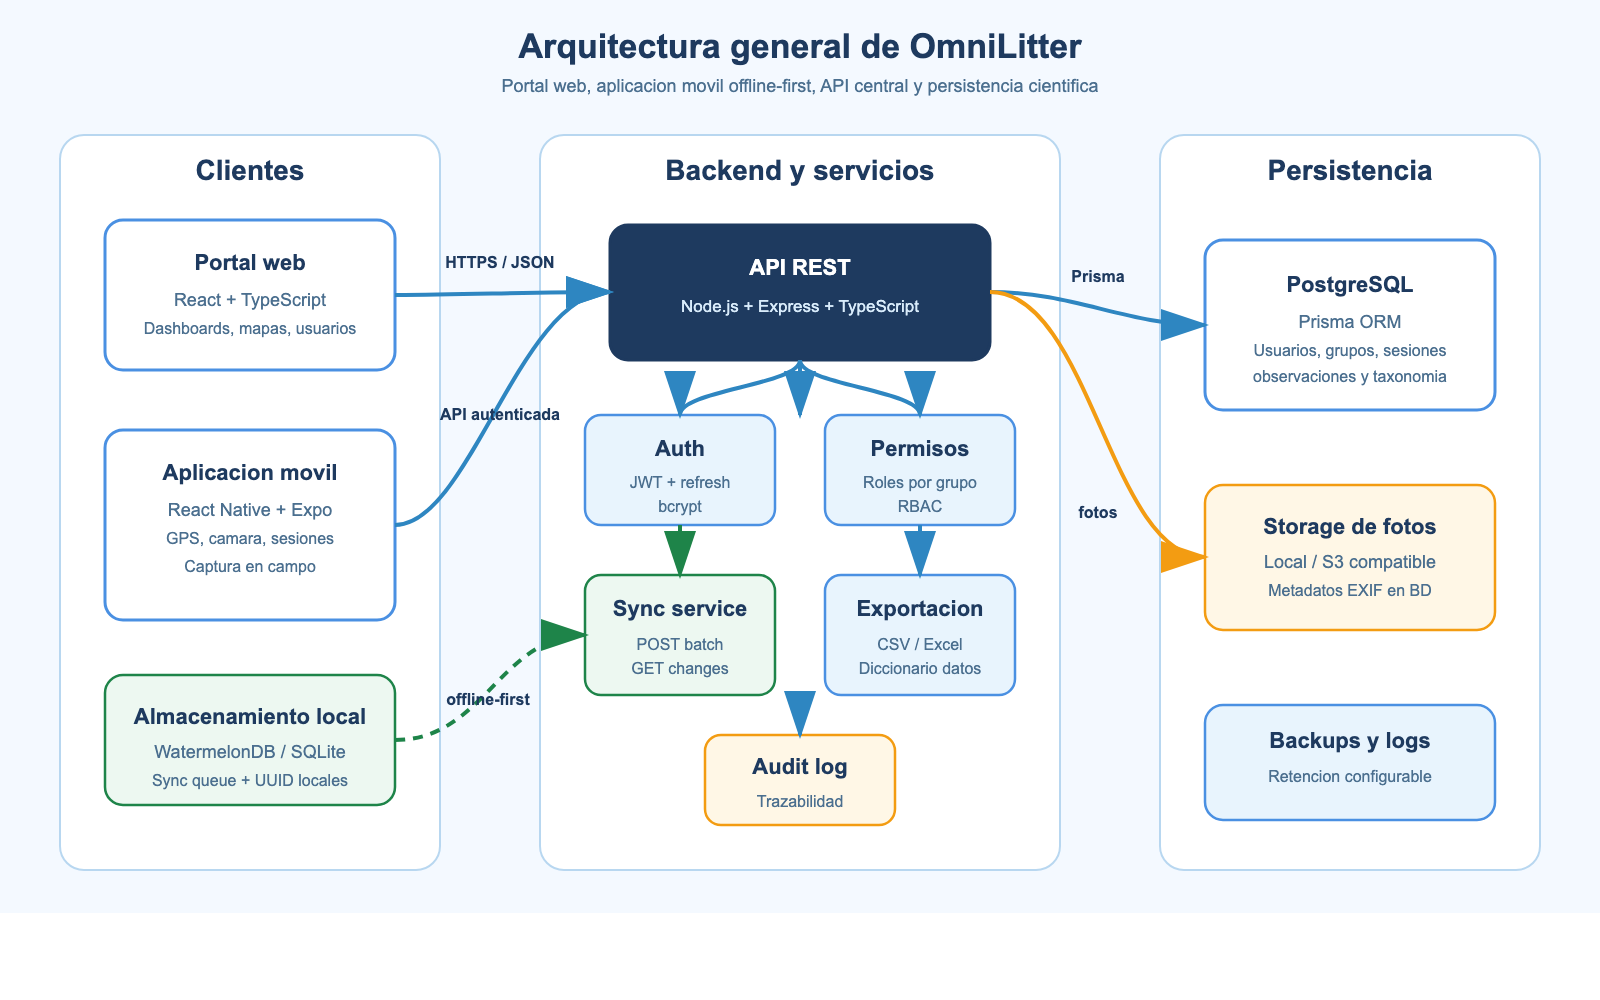
\includegraphics[width=0.8\textwidth]{figures/arquitectura.png}
  \caption{Arquitectura general propuesta para OmniLitter.}
  \label{fig:arquitectura}
\end{figure}


\subsubsection{Justificación de las decisiones arquitectónicas principales}

\textbf{API REST como único punto de acceso.}
Centralizar la lógica de negocio en la API evita duplicidades entre los dos clientes y
facilita la incorporación de nuevos consumidores en el futuro (p.ej., exportaciones
automatizadas por \textit{scripts} externos o integraciones con repositorios científicos).

\textbf{Separación entre portal web y aplicación móvil.}
Aunque comparten la misma API, los dos clientes tienen requisitos de experiencia de usuario
muy distintos: el portal prioriza la visualización analítica y la gestión, mientras que la
app móvil prioriza la captura rápida en condiciones de campo adversas (luz solar, guantes,
sin conexión). Mantenerlos como proyectos independientes permite evolucionar cada uno a su
propio ritmo.

\textbf{Base de datos local en el móvil.}
El trabajo de campo se realiza habitualmente en zonas costeras, ribereñas o forestales
con cobertura de red intermitente o nula. La decisión de embeber una base de datos local en
el dispositivo es, por tanto, un requisito no negociable para la viabilidad del producto.

% ------------------------------------------------------------
\subsection{Diseño de la Base de Datos}
% ------------------------------------------------------------

\subsubsection{Modelo relacional}

El modelo de datos de OmniLitter se compone de once entidades que se agrupan en tres
áreas funcionales:

\begin{itemize}
  \item \textbf{Gestión de acceso:} \texttt{USER}, \texttt{GROUP}, \texttt{MEMBERSHIP}.
  \item \textbf{Organización científica:} \texttt{CAMPAIGN}, \texttt{SURVEY\_SESSION}.
  \item \textbf{Datos de campo:} \texttt{OBSERVATION}, \texttt{PHOTO},
    \texttt{TAXONOMY\_ITEM}, \texttt{FAVORITE}, \texttt{AUDIT\_LOG}.
\end{itemize}

La figura~\ref{fig:modelo_er} muestra el diagrama entidad-relación del sistema.

\begin{figure}[H]
  \centering
  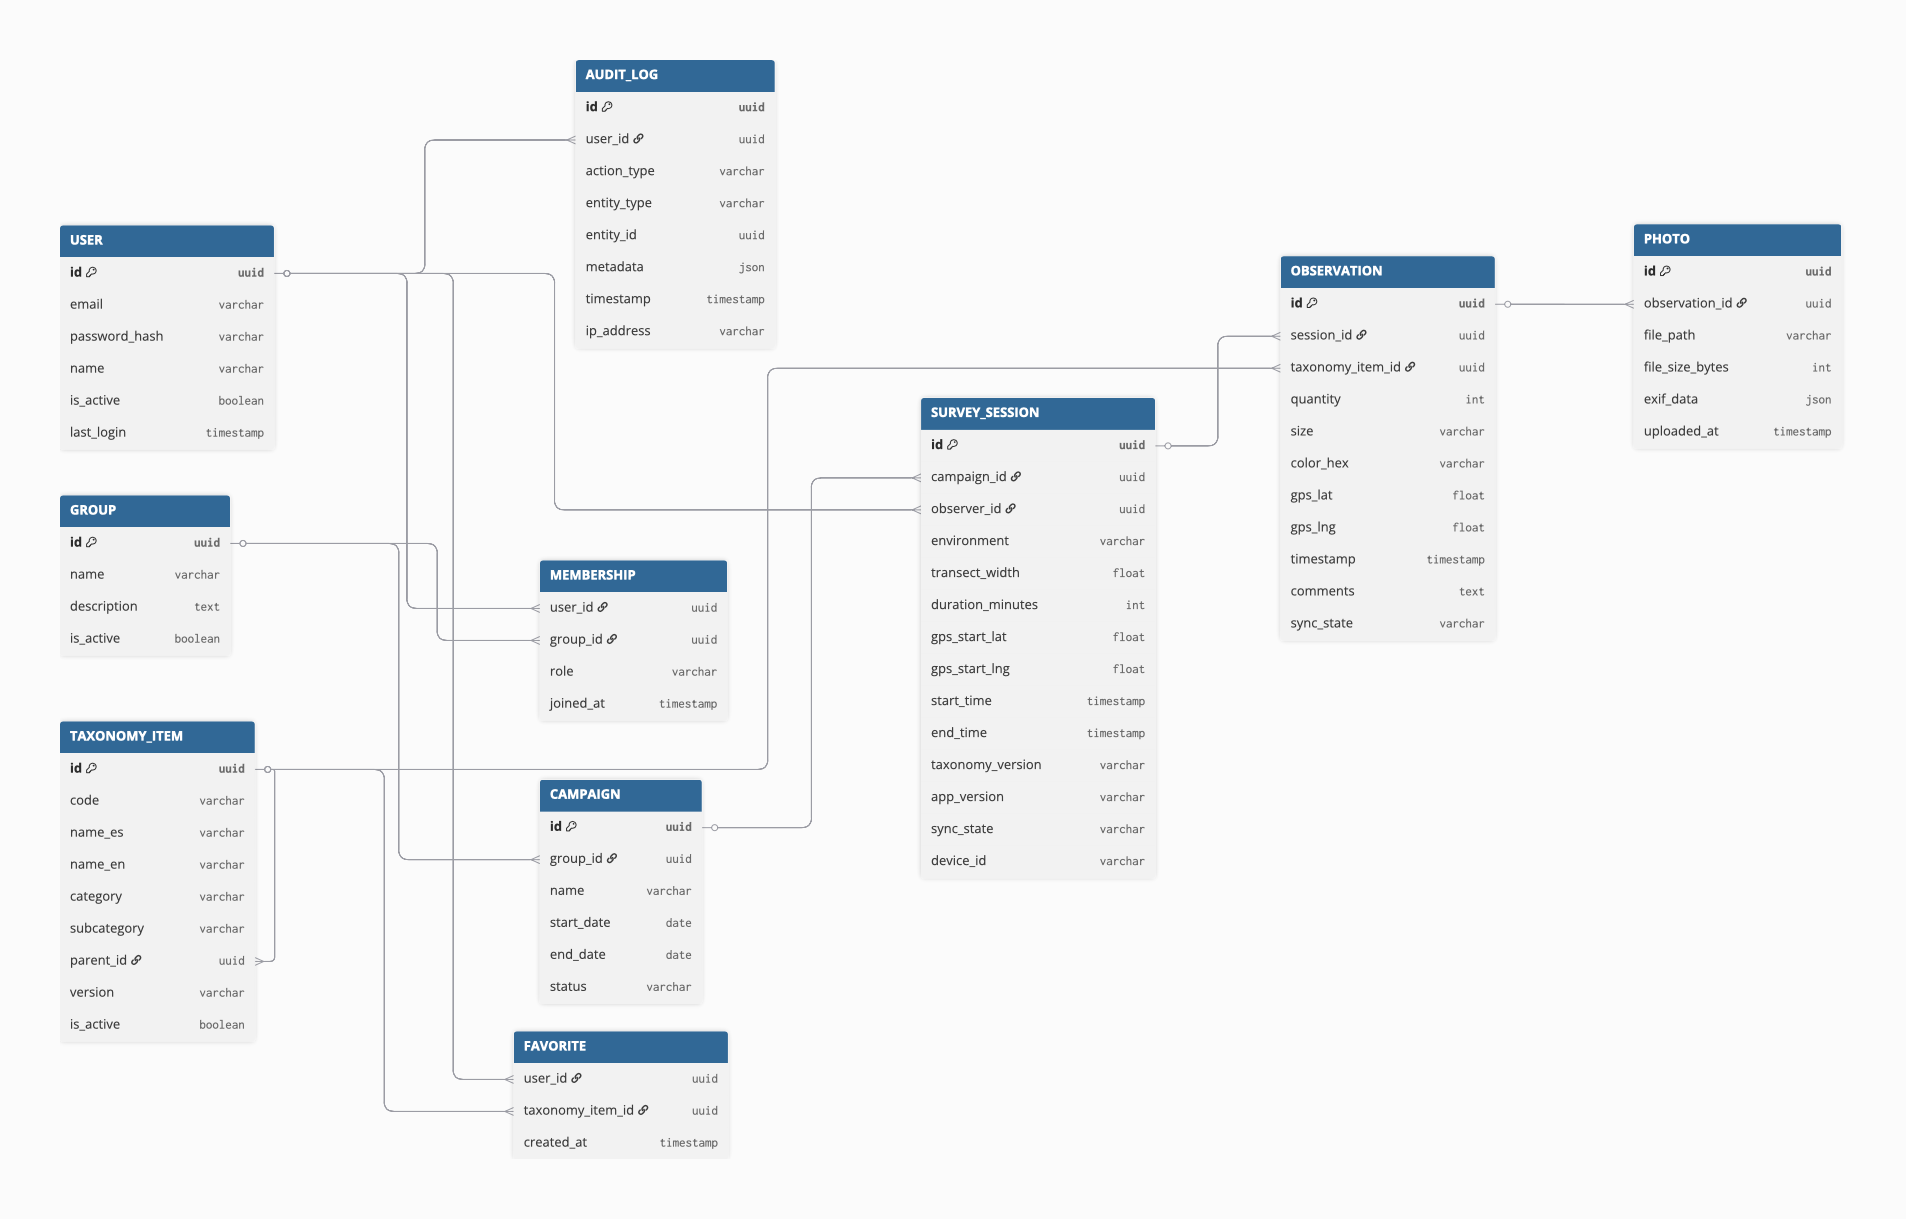
\includegraphics[width=\textwidth]{figures/modelo_er.png}
  \caption{Diagrama entidad-relación del sistema OmniLitter.}
  \label{fig:modelo_er}
\end{figure}


\subsubsection{Descripción de entidades}

La tabla~\ref{tab:entidades} describe los atributos clave de cada entidad y su
propósito en el sistema.

\begin{longtable}{p{3.2cm} p{4.2cm} p{6.6cm}}
  \caption{Descripción de entidades del modelo de datos.}
  \label{tab:entidades} \\
  \toprule
  \textbf{Entidad} & \textbf{Atributos principales} & \textbf{Descripción} \\
  \midrule
  \endfirsthead
  \toprule
  \textbf{Entidad} & \textbf{Atributos principales} & \textbf{Descripción} \\
  \midrule
  \endhead
  \bottomrule
  \endfoot

  \texttt{USER} &
    \texttt{id (UUID)}, \texttt{email}, \texttt{password\_hash}, \texttt{name},
    \texttt{is\_active}, \texttt{last\_login} &
    Representa a cada persona registrada en el sistema. Las contraseñas se almacenan
    como \textit{hash} bcrypt y nunca en texto plano. \\[4pt]

  \texttt{GROUP} &
    \texttt{id (UUID)}, \texttt{name}, \texttt{description}, \texttt{is\_active} &
    Equipo de investigación. Un grupo puede ser archivado sin eliminar sus datos
    históricos, preservando la trazabilidad científica. \\[4pt]

  \texttt{MEMBERSHIP} &
    \texttt{user\_id (FK)}, \texttt{group\_id (FK)},
    \texttt{role (admin|editor|viewer)}, \texttt{joined\_at} &
    Tabla de unión que asocia usuarios con grupos asignándoles un rol. Un mismo usuario
    puede tener roles distintos en grupos distintos. \\[4pt]

  \texttt{CAMPAIGN} &
    \texttt{id (UUID)}, \texttt{group\_id (FK)}, \texttt{name},
    \texttt{start\_date}, \texttt{end\_date}, \texttt{status} &
    Proyecto científico de muestreo. Agrupa varias sesiones de campo bajo un
    objetivo común (p.ej., «Monitoreo anual Playa de la Caleta 2026»). \\[4pt]

  \texttt{SURVEY\_SESSION} &
    \texttt{id (UUID)}, \texttt{campaign\_id (FK)}, \texttt{observer\_id (FK)},
    \texttt{environment}, \texttt{transect\_width}, \texttt{duration\_minutes},
    \texttt{gps\_start\_lat/lng}, \texttt{start\_time}, \texttt{end\_time},
    \texttt{taxonomy\_version}, \texttt{app\_version}, \texttt{sync\_state},
    \texttt{device\_id} &
    Sesión de muestreo individual en campo. Registra todos los metadatos científicos
    necesarios para la reproducibilidad: protocolo, versión de taxonomía utilizada y
    versión de la aplicación. El campo \texttt{sync\_state} gestiona el ciclo de vida
    de la sincronización. \\[4pt]

  \texttt{OBSERVATION} &
    \texttt{id (UUID)}, \texttt{session\_id (FK)},
    \texttt{taxonomy\_item\_id (FK)}, \texttt{quantity}, \texttt{size},
    \texttt{color\_hex}, \texttt{gps\_lat/lng}, \texttt{timestamp},
    \texttt{comments}, \texttt{sync\_state} &
    Registro de un ítem de residuo observado. Constituye la unidad mínima de dato
    científico del sistema. \\[4pt]

  \texttt{PHOTO} &
    \texttt{id (UUID)}, \texttt{observation\_id (FK)}, \texttt{file\_path},
    \texttt{file\_size\_bytes}, \texttt{exif\_data (JSONB)}, \texttt{uploaded\_at} &
    Imagen asociada a una observación. Los metadatos EXIF (coordenadas GPS
    embebidas en la imagen, fecha de captura, modelo de cámara) se almacenan en
    formato JSONB para máxima flexibilidad. \\[4pt]

  \texttt{TAXONOMY\_ITEM} &
    \texttt{id (UUID)}, \texttt{code}, \texttt{name\_es}, \texttt{name\_en},
    \texttt{category}, \texttt{subcategory}, \texttt{parent\_id (FK self-ref)},
    \texttt{version}, \texttt{is\_active} &
    Catálogo de tipos de residuo basado en la \textit{Joint List of Litter Categories}.
    La estructura jerárquica autorreferenciada (categoría → subcategoría → ítem)
    permite navegar la taxonomía sin conexión, ya que se descarga completa
    al iniciar sesión. \\[4pt]

  \texttt{FAVORITE} &
    \texttt{user\_id (FK)}, \texttt{taxonomy\_item\_id (FK)}, \texttt{created\_at} &
    Ítems de taxonomía marcados como favoritos por el usuario para agilizar la
    captura de observaciones en campo. \\[4pt]

  \texttt{AUDIT\_LOG} &
    \texttt{id}, \texttt{user\_id (FK)}, \texttt{action\_type},
    \texttt{entity\_type}, \texttt{entity\_id}, \texttt{metadata (JSONB)},
    \texttt{timestamp}, \texttt{ip\_address} &
    Registro de auditoría que almacena las acciones relevantes sobre el sistema
    (inicio de sesión, creación y edición de observaciones, exportaciones de datos,
    cambios de configuración). Garantiza la trazabilidad exigida en entornos de
    investigación científica. \\

\end{longtable}

\subsubsection{Decisiones de diseño de la base de datos}

\textbf{UUID como clave primaria universal.}
Todos los identificadores primarios son UUID v4 generados en el cliente (ya sea el
navegador o el dispositivo móvil). Esto resuelve el problema de colisiones de claves
en escenarios de creación offline: dos dispositivos diferentes que creen una observación
sin conexión obtendrán identificadores globalmente únicos que no entrarán en conflicto
cuando se sincronicen con el servidor.

\textbf{Rol en \texttt{MEMBERSHIP}, no en \texttt{USER}.}
El rol de un investigador no es una propiedad intrínseca de la persona, sino de su
relación con un grupo concreto. Un mismo investigador puede ser administrador en su
grupo principal y colaborador invitado en otro grupo. Modelar el rol en la tabla de
unión es, por tanto, la decisión correcta desde el punto de vista semántico.

\textbf{Versión de taxonomía en cada sesión y observación.}
La taxonomía de residuos evoluciona con el tiempo a medida que la comunidad científica
añade o reorganiza categorías. Registrar la versión exacta utilizada en cada sesión
permite reconstruir con exactitud qué definición se aplicó a cada observación, lo que
es un requisito básico de reproducibilidad científica.

\textbf{JSONB para metadatos heterogéneos.}
Los campos \texttt{exif\_data} y \texttt{metadata} utilizan el tipo JSONB de PostgreSQL
para almacenar datos cuya estructura puede variar (distintos modelos de cámara incluyen
campos EXIF diferentes, distintas acciones de auditoría tienen distintos contextos).
Esta decisión evita la proliferación de columnas opcionales con valor nulo y preserva
la flexibilidad para añadir nuevos atributos sin migrar el esquema.

% ------------------------------------------------------------
\subsection{Diseño de la API REST}
% ------------------------------------------------------------

La API sigue los principios REST: interfaz uniforme, comunicación sin estado,
recursos identificados por URI y representaciones en formato JSON. Todos los
\textit{endpoints} protegidos requieren el encabezado
\texttt{Authorization: Bearer <token>}, donde el \textit{token} es un JWT firmado
emitido en el \textit{endpoint} de autenticación.

La tabla~\ref{tab:endpoints} recoge los \textit{endpoints} principales agrupados
por recurso.

\begin{longtable}{p{1.5cm} p{5.5cm} p{2cm} p{4cm}}
  \caption{Principales \textit{endpoints} de la API REST de OmniLitter.}
  \label{tab:endpoints} \\
  \toprule
  \textbf{Método} & \textbf{Ruta} & \textbf{Protegido} & \textbf{Descripción} \\
  \midrule
  \endfirsthead
  \toprule
  \textbf{Método} & \textbf{Ruta} & \textbf{Protegido} & \textbf{Descripción} \\
  \midrule
  \endhead
  \bottomrule
  \endfoot

  \multicolumn{4}{l}{\textit{Autenticación}} \\[2pt]
  POST & \texttt{/api/auth/login} & No & Emite JWT de acceso y refresco \\
  POST & \texttt{/api/auth/refresh} & No & Renueva el JWT de acceso \\
  POST & \texttt{/api/auth/logout} & Sí & Invalida el \textit{token} de refresco \\[6pt]

  \multicolumn{4}{l}{\textit{Usuarios}} \\[2pt]
  GET  & \texttt{/api/users} & Sí (admin) & Lista todos los usuarios \\
  POST & \texttt{/api/users} & Sí (admin) & Crea un nuevo usuario \\
  GET  & \texttt{/api/users/:id} & Sí & Obtiene un usuario \\
  PATCH & \texttt{/api/users/:id} & Sí (admin) & Actualiza datos o estado \\[6pt]

  \multicolumn{4}{l}{\textit{Grupos}} \\[2pt]
  GET  & \texttt{/api/groups} & Sí & Lista grupos del usuario autenticado \\
  POST & \texttt{/api/groups} & Sí (admin) & Crea un grupo \\
  PATCH & \texttt{/api/groups/:id} & Sí (admin) & Edita nombre/descripción \\
  DELETE & \texttt{/api/groups/:id/archive} & Sí (admin) & Archiva un grupo \\
  POST & \texttt{/api/groups/:id/members} & Sí (admin) & Añade miembro \\
  DELETE & \texttt{/api/groups/:id/members/:uid} & Sí (admin) & Elimina miembro \\[6pt]

  \multicolumn{4}{l}{\textit{Sesiones de muestreo}} \\[2pt]
  GET  & \texttt{/api/sessions} & Sí & Lista sesiones accesibles \\
  POST & \texttt{/api/sessions} & Sí & Crea una sesión \\
  GET  & \texttt{/api/sessions/:id} & Sí & Obtiene una sesión con observaciones \\
  PATCH & \texttt{/api/sessions/:id} & Sí & Actualiza metadatos \\[6pt]

  \multicolumn{4}{l}{\textit{Observaciones}} \\[2pt]
  GET  & \texttt{/api/sessions/:id/observations} & Sí & Lista observaciones de sesión \\
  POST & \texttt{/api/sessions/:id/observations} & Sí & Registra una observación \\
  GET  & \texttt{/api/observations} & Sí & Lista todas (filtros opcionales) \\[6pt]

  \multicolumn{4}{l}{\textit{Fotos}} \\[2pt]
  POST & \texttt{/api/observations/:id/photos} & Sí & Sube una foto (multipart) \\
  GET  & \texttt{/api/photos/:id} & Sí & Sirve el archivo de imagen \\[6pt]

  \multicolumn{4}{l}{\textit{Taxonomía}} \\[2pt]
  GET  & \texttt{/api/taxonomy} & Sí & Descarga la taxonomía completa \\
  GET  & \texttt{/api/taxonomy?version=:v} & Sí & Descarga versión específica \\[6pt]

  \multicolumn{4}{l}{\textit{Sincronización}} \\[2pt]
  POST & \texttt{/api/sync/batch} & Sí & Sube cola de registros pendientes \\
  GET  & \texttt{/api/sync/changes} & Sí & Descarga cambios desde \texttt{last\_sync} \\[6pt]

  \multicolumn{4}{l}{\textit{Exportación}} \\[2pt]
  GET  & \texttt{/api/export/csv} & Sí (admin) & Exporta observaciones en CSV científico \\

\end{longtable}

\subsubsection{Autenticación y autorización}

El sistema implementa autenticación basada en JWT con dos \textit{tokens}: un
\textbf{token de acceso} de corta duración (15 minutos) y un \textbf{token de refresco}
de larga duración (7 días). El token de acceso se envía en cada petición en el encabezado
\texttt{Authorization}; el de refresco se utiliza exclusivamente para solicitar un nuevo
token de acceso cuando el anterior expira.

La autorización sigue un modelo de control de acceso basado en roles (RBAC)
a nivel de grupo. El \textit{middleware} de autorización verifica, para cada petición,
que el usuario autenticado posee el rol requerido en el grupo al que pertenece el
recurso solicitado. Esto permite que una misma persona sea administradora en un grupo
y colaboradora en otro, con permisos diferentes en cada contexto.

% ------------------------------------------------------------
\subsection{Diseño del Portal Web}
% ------------------------------------------------------------

\subsubsection{Arquitectura de componentes}

El portal web está implementado como una \textit{Single Page Application} (SPA) con
React 18 y TypeScript, empaquetada con Vite y estilizada con Tailwind CSS. La
navegación entre páginas es gestionada por React Router, que define dos niveles de rutas:

\begin{itemize}
  \item \textbf{Rutas públicas:} la página de inicio (\texttt{/}) y el formulario
    de inicio de sesión (\texttt{/login}), accesibles sin autenticación.
  \item \textbf{Rutas protegidas:} todas las páginas bajo \texttt{/app/*}, protegidas
    por un componente \texttt{PrivateRoute} que verifica el estado de autenticación y
    redirige al \textit{login} si no existe sesión activa.
\end{itemize}

La estructura de componentes sigue una jerarquía de tres niveles: el \texttt{Layout}
general (barra lateral, encabezado, selector de grupo activo) envuelve las páginas
individuales, que a su vez utilizan componentes reutilizables (tarjetas de estadística,
tablas filtrables, modales de confirmación).

\subsubsection{Gestión de estado}

El portal web utiliza \texttt{localStorage} como mecanismo de persistencia de la
sesión del usuario entre recargas de página, almacenando el JWT de acceso, el nombre
del usuario, su rol y el grupo activo seleccionado. Este enfoque es suficiente para
una SPA sin estado de servidor, y se complementará con manejo de \textit{refresh
token} en la implementación real.

La comunicación entre el selector de grupo activo (ubicado en la barra lateral) y el
componente Dashboard se implementa mediante un evento personalizado del DOM
(\texttt{omnilitter:groupChanged}), lo que evita prop-drilling innecesario sin
requerir una solución de gestión de estado global.

\subsubsection{Flujo de navegación y control de acceso por rol}

Las secciones de \textbf{Grupos} y \textbf{Usuarios} son exclusivas del rol de
administrador y no aparecen en la barra de navegación para los colaboradores.
El Dashboard ajusta el contenido mostrado según el rol: los administradores ven
estadísticas globales del grupo activo, mientras que los colaboradores ven únicamente
sus propias métricas. La tabla de observaciones filtra los registros por autor para los
colaboradores y muestra todos para los administradores.

% ------------------------------------------------------------
\subsection{Diseño de la Aplicación Móvil}
% ------------------------------------------------------------

\subsubsection{Stack tecnológico y estructura de pantallas}

La aplicación móvil está construida con \textbf{React Native} y \textbf{Expo bare
workflow}. La elección del \textit{bare workflow} frente al \textit{managed workflow}
responde a la necesidad de acceso completo a las APIs nativas del dispositivo: GPS
continuo con expo-location, captura de imagen con metadatos EXIF con expo-camera,
y sincronización en segundo plano con expo-background-fetch.

La navegación está organizada en dos niveles:

\begin{itemize}
  \item \textbf{Navegación de primer nivel (tab bar):} cinco pestañas inferiores
    (Inicio, Sesiones, Mapa, Sincronización, Perfil), visibles únicamente en las
    pantallas principales.
  \item \textbf{Navegación de pila (\textit{stack}):} flujos de varios pasos como la
    creación de una nueva sesión o la captura de una observación, que se presentan
    sin el \textit{tab bar}.
\end{itemize}

\subsubsection{Gestión de estado global}

El estado global de la aplicación se gestiona mediante el patrón
\textbf{Context + useReducer} de React, sin dependencias externas de gestión de
estado. El contexto \texttt{AppContext} expone el estado completo (sesiones activas,
tipos de residuo, datos del usuario, estado de sincronización) y un \textit{dispatcher}
con acciones tipadas en TypeScript. Este patrón proporciona la predictibilidad de
Redux con una superficie de código significativamente menor, adecuada para la escala
del proyecto.

\subsubsection{Base de datos local con WatermelonDB}

WatermelonDB actúa como base de datos local sobre SQLite. Se elige frente a SQLite
directo por tres razones: (1) está diseñado explícitamente para el patrón
\textit{offline-first} con sincronización en diferido; (2) ofrece un sistema de
consultas reactivo basado en observables que actualiza la UI automáticamente cuando
cambian los datos; (3) su rendimiento en colecciones grandes (miles de observaciones)
es significativamente superior al de SQLite gestionado manualmente.

El esquema local replica el subconjunto del modelo de datos necesario para la
operación en campo: \texttt{survey\_sessions}, \texttt{observations}, \texttt{photos}
y \texttt{sync\_queue}, además de la taxonomía completa cargada al iniciar sesión.

\subsubsection{Flujo de captura de una observación}

El flujo principal de la aplicación sigue esta secuencia:

\begin{enumerate}
  \item El investigador inicia una nueva sesión de muestreo, especificando el nombre,
    el tipo de entorno y los parámetros del transecto.
  \item Para cada ítem encontrado, abre la pantalla de nueva observación, selecciona
    el tipo de residuo a través del modal de taxonomía (organizado en cuadrícula visual
    por categorías e iconos), e introduce cantidad, tamaño, color y comentarios.
  \item Opcionalmente captura una foto geolocalizada del residuo.
  \item Al finalizar la sesión de campo, revisa el resumen y puede iniciar la
    sincronización manualmente o dejar que se realice en segundo plano al recuperar
    cobertura de red.
\end{enumerate}

% ------------------------------------------------------------
\subsection{Mecanismo de Sincronización Offline}
% ------------------------------------------------------------

\subsubsection{Patrón Outbox Queue}

El mecanismo de sincronización implementa el patrón \textbf{Outbox Queue}
(cola de salida), ampliamente utilizado en sistemas distribuidos con conectividad
intermitente. El funcionamiento es el siguiente:

\begin{enumerate}
  \item Cuando el usuario crea o modifica un registro (sesión u observación) en el
    dispositivo sin conexión, el registro se persiste en WatermelonDB con
    \texttt{sync\_state = PENDING} y se inserta una entrada en la tabla
    \texttt{sync\_queue} con el \textit{payload} completo del cambio.
  \item Cuando el dispositivo recupera conectividad, \texttt{expo-background-fetch}
    activa el proceso de sincronización, que lee la cola y realiza una petición
    \texttt{POST /api/sync/batch} con todos los registros pendientes.
  \item El servidor procesa los registros en orden, los persiste en PostgreSQL y
    devuelve el estado canónico actualizado.
  \item El cliente actualiza el \texttt{sync\_state} de los registros procesados a
    \texttt{SYNCED} y descarga los cambios remotos realizados por otros usuarios
    mediante \texttt{GET /api/sync/changes?since=\{last\_sync\_timestamp\}}.
  \item En caso de error en un registro concreto (conflicto de datos, registro
    inválido), ese registro pasa a \texttt{sync\_state = ERROR} y se notifica al
    usuario, sin bloquear la sincronización del resto.
\end{enumerate}

\subsubsection{Estados de sincronización}

Cada sesión y observación puede encontrarse en uno de cuatro estados, como muestra
la tabla~\ref{tab:sync_states}.

\begin{table}[H]
  \centering
  \caption{Estados de sincronización y su significado.}
  \label{tab:sync_states}
  \begin{tabularx}{\textwidth}{lX}
    \toprule
    \textbf{Estado} & \textbf{Significado} \\
    \midrule
    \texttt{PENDING}  & El registro existe solo en el dispositivo; aún no se ha
                        intentado sincronizar. \\
    \texttt{SYNCING}  & El registro está siendo procesado en la petición de
                        sincronización actual. \\
    \texttt{SYNCED}   & El servidor ha confirmado la recepción y persistencia del
                        registro. \\
    \texttt{ERROR}    & El servidor rechazó el registro (conflicto, datos inválidos).
                        Requiere intervención manual o reintento. \\
    \bottomrule
  \end{tabularx}
\end{table}

\subsubsection{Resolución de conflictos}

La estrategia de resolución de conflictos adoptada es \textbf{last-write-wins} con
granularidad de registro: si dos usuarios modifican la misma sesión de forma
independiente mientras están sin conexión, prevalece la versión con el
\texttt{timestamp} más reciente. Esta estrategia es suficiente para el modelo de uso
de OmniLitter, donde cada sesión de muestreo pertenece a un único observador
responsable y los conflictos genuinos son infrecuentes.

\subsubsection{Garantía de identificadores únicos en entorno offline}

Para que la estrategia Outbox Queue funcione sin servidor central asignando IDs,
todos los identificadores del sistema son \textbf{UUID v4 generados en el cliente}.
Esto garantiza que los registros creados simultáneamente en distintos dispositivos
nunca colisionarán al sincronizarse, independientemente del orden de llegada al
servidor.

\newpage

\chapter{Desarrollo, implantación y validación}
\label{sec:desarrollo_implantacion_validacion}

\section{Organización del desarrollo}
\subsection{Metodología de trabajo}
\subsection{Gestión del proyecto en GitHub Projects}
\subsection{Plan de pruebas}

La validación del proyecto se organizó de forma incremental, siguiendo la misma división por sprints utilizada durante el desarrollo. El objetivo fue comprobar, en cada etapa, que las funcionalidades incorporadas no solo estaban disponibles desde la interfaz, sino que respetaban las reglas de negocio, los permisos, los contratos de datos y las restricciones definidas para el sistema.

La estrategia de pruebas combinó dos enfoques complementarios. Por un lado, se implementaron pruebas automatizadas sobre las partes más críticas del proyecto: esquemas compartidos, servicios de la API y determinadas utilidades del portal web. Por otro lado, los recorridos completos de usuario, especialmente aquellos relacionados con la aplicación móvil, el uso offline, la cámara, la ubicación y la sincronización, se validaron mediante pruebas manuales funcionales apoyadas en evidencias visuales.

Esta separación permite reflejar con precisión el alcance real de la validación. La memoria no atribuye al proyecto pruebas automatizadas que no existen, pero sí deja constancia de que las funcionalidades principales fueron comprobadas mediante el tipo de prueba más adecuado a su naturaleza.

\begin{table}[H]
\centering
\caption{Estrategia general de pruebas del proyecto}
\label{tab:estrategia_general_pruebas}
\small
\begin{tabularx}{\textwidth}{p{3.2cm}X X}
\toprule
Tipo de prueba & Objetivo & Aplicación en OmniLitter \\
\midrule
Pruebas de contrato & Verificar que los datos intercambiados entre clientes y API cumplen la estructura esperada. & Esquemas compartidos de autenticación, campañas, catálogo, sesiones, observaciones y fotografías. \\
Pruebas unitarias de servicio & Comprobar reglas de negocio sin depender de la interfaz ni de una base de datos real. & Servicios de usuarios, grupos, campañas, catálogo y observaciones del backend mediante mocks de Prisma. \\
Pruebas automatizadas web & Validar lógica auxiliar del portal web que no depende directamente de componentes visuales. & Cálculo de distancia de rutas y preferencias de exportación del dashboard. \\
Pruebas manuales funcionales & Comprobar recorridos completos desde la perspectiva del usuario final. & Portal web, aplicación móvil, captura de campo, uso offline, sincronización y evidencias visuales. \\
Pruebas de regresión & Comprobar que los cambios posteriores no rompen funcionalidades ya validadas. & Reejecución de la suite automatizada y revisión manual de los flujos principales al cierre de cada sprint. \\
\bottomrule
\end{tabularx}
\end{table}

La suite automatizada se ejecutó con \textit{Vitest}. En el paquete compartido se utilizaron esquemas definidos con \textit{Zod}, mientras que en el backend se validaron servicios mediante mocks de Prisma. Esta decisión permitió comprobar reglas de negocio relevantes sin depender de una base de datos PostgreSQL real ni de la ejecución completa de rutas HTTP.

\begin{table}[H]
\centering
\caption{Alcance real de las pruebas automatizadas}
\label{tab:alcance_real_pruebas_automatizadas}
\small
\begin{tabularx}{\textwidth}{p{2.4cm}p{3.4cm}p{2.4cm}X}
\toprule
Área & Ficheros implementados & Herramienta & Cobertura principal \\
\midrule
API & Tests de \texttt{apps/api} & Vitest & Servicios de campañas, catálogo, grupos, usuarios y observaciones con mocks de Prisma. \\
Web & Tests de \texttt{apps/web} & Vitest & Preferencias de exportación del dashboard y cálculo de distancia de rutas. \\
Shared & Test de \texttt{packages/shared} & Vitest + Zod & Esquemas compartidos de autenticación, campañas, catálogo, sesiones, observaciones y fotografías. \\
Mobile & Sin ficheros de test configurados & No aplica & La aplicación móvil se validó mediante pruebas manuales funcionales y evidencias visuales. \\
\bottomrule
\end{tabularx}
\end{table}

Para facilitar la trazabilidad, las pruebas automatizadas se agruparon mediante códigos identificativos. Estos códigos se emplean en los apartados de cada sprint para relacionar las tareas desarrolladas con las comprobaciones realizadas.

\begin{table}[H]
\centering
\caption{Leyenda de códigos usados en las pruebas}
\label{tab:leyenda_codigos_pruebas}
\small
\begin{tabularx}{\textwidth}{p{2.7cm}X}
\toprule
Código & Significado \\
\midrule
SCH & Pruebas de contrato sobre esquemas compartidos. Validan que los datos enviados por web, móvil o API cumplen la estructura esperada. \\
USR & Pruebas del servicio de usuarios del backend. \\
GRP & Pruebas del servicio de grupos y membresías del backend. \\
CMP & Pruebas del servicio de campañas del backend. \\
CAT & Pruebas del catálogo científico usado por el sistema. \\
OBS & Pruebas del servicio de observaciones del backend. \\
WEB-SES & Pruebas de utilidades web relacionadas con sesiones y cálculo de distancias. \\
WEB-EXP & Pruebas de preferencias de exportación en el portal web. \\
\bottomrule
\end{tabularx}
\end{table}

La ejecución global de la suite automatizada finalizó correctamente. En total se ejecutaron 77 pruebas automatizadas distribuidas entre el paquete compartido, el portal web y la API.

\begin{table}[H]
\centering
\caption{Resultado global de la ejecución de pruebas automatizadas}
\label{tab:resultado_global_pruebas_automatizadas}
\small
\begin{tabularx}{\textwidth}{p{4cm}p{4cm}r r}
\toprule
Paquete & Resultado & Ficheros & Casos \\
\midrule
\texttt{@omnilitter/shared} & Correcto & 1 & 23 \\
\texttt{@omnilitter/web} & Correcto & 2 & 15 \\
\texttt{@omnilitter/api} & Correcto & 5 & 39 \\
\texttt{@omnilitter/mobile} & Sin tests automatizados configurados & 0 & 0 \\
\midrule
Total ejecutado & Correcto & 8 & 77 \\
\bottomrule
\end{tabularx}
\end{table}

\subsection{Criterios de finalización de tareas}
\subsection{Estructura de releases}

\clearpage
\section{Sprint 1: Base funcional del sistema}
\subsection{Objetivo del sprint}
\subsection{Parte del proyecto abordada}
\subsection{Tiempo invertido y reparto del trabajo}
\subsection{Implementación realizada}
\subsection{Pruebas realizadas}

En el primer sprint se validó la base funcional del sistema. Las pruebas se centraron en autenticación, administración inicial de usuarios y grupos, campañas, catálogo, sesiones de muestreo y primeras observaciones. Esta fase era especialmente importante porque establecía los contratos y servicios sobre los que se apoyarían los sprints posteriores.

\subsubsection{Pruebas automatizadas implementadas}

\begin{table}[H]
\centering
\caption{Pruebas automatizadas vinculadas al Sprint 1}
\label{tab:pruebas_automatizadas_sprint1}
\scriptsize
\begin{tabularx}{\textwidth}{p{3.5cm}p{3cm}X p{1.8cm}}
\toprule
Tarea o funcionalidad & Cobertura automatizada & Comprobación principal & Resultado \\
\midrule
Login, registro y cierre de sesión & SCH-01, SCH-02 & Validación del registro con contraseña robusta, confirmación coincidente y rechazo de contraseñas débiles o confirmaciones incorrectas. & Correcto \\
Portal de administración de usuarios & USR-01, USR-03 & Bloqueo de correos duplicados y creación de usuarios con o sin membresías iniciales. & Correcto \\
Gestión de grupos y membresías & GRP-06, GRP-07 & Restauración de grupos, permisos de administración y rechazo de acciones realizadas por usuarios sin autorización. & Correcto \\
Campañas y sesiones backend & SCH-04 a SCH-13, CMP-01 & Estados válidos de campañas, referencias de catálogo y reglas de geometría para sesiones libres, por cuadrícula o por transecto. & Correcto \\
Catálogo científico & CAT-01 a CAT-08 & Creación, actualización, detección de duplicados, borrado y restricciones por uso de entornos y tipologías. & Correcto \\
API de observaciones y adjuntos & SCH-14 a SCH-23, OBS-04 a OBS-06 & Observaciones con ítems obligatorios, coordenadas válidas, cantidades positivas, tipos de imagen soportados y control de acceso a observaciones propias o ajenas. & Correcto \\
Formulario móvil de observación & SCH-14 a SCH-16 & Validación compartida de sesión, taxonomía, coordenadas, ítems y cantidades utilizada por el formulario móvil. & Correcto \\
\bottomrule
\end{tabularx}
\end{table}

Estas pruebas protegen reglas que no deben depender únicamente de la interfaz. Aunque los formularios ayuden a evitar datos incorrectos, los esquemas compartidos y los servicios de backend garantizan que la validación se mantiene ante datos reutilizados por distintos clientes o enviados directamente a la API.

\subsubsection{Pruebas manuales funcionales}

Las pruebas manuales de este sprint se reservan para los recorridos completos de usuario, como registro, inicio de sesión, administración básica, creación de campañas, creación de sesiones y registro inicial de observaciones desde la aplicación móvil. Su detalle se documenta mediante evidencias visuales en el apartado correspondiente de validación manual.

\subsection{Desviaciones e incidencias}
\subsection{Resultado del sprint}

\clearpage
\section{Sprint 2: Captura de campo y análisis inicial}
\subsection{Objetivo del sprint}
\subsection{Parte del proyecto abordada}
\subsection{Tiempo invertido y reparto del trabajo}
\subsection{Implementación realizada}
\subsection{Pruebas realizadas}

El segundo sprint reforzó la captura de datos de campo y el análisis inicial. La validación se orientó a comprobar la calidad del dato capturado, la incorporación de fotografías, el uso de ubicación GPS, el control de permisos sobre observaciones y las primeras funcionalidades de análisis del portal web.

\subsubsection{Pruebas automatizadas implementadas}

\begin{table}[H]
\centering
\caption{Pruebas automatizadas vinculadas al Sprint 2}
\label{tab:pruebas_automatizadas_sprint2}
\scriptsize
\begin{tabularx}{\textwidth}{p{3.5cm}p{3cm}X p{1.8cm}}
\toprule
Tarea o funcionalidad & Cobertura automatizada & Comprobación principal & Resultado \\
\midrule
GPS en sesión y observación & WEB-SES-01 a WEB-SES-03 & Cálculo de distancia para rutas vacías, rutas con un único punto y suma de distancia Haversine entre puntos consecutivos. & Correcto \\
Fotografías por observación y metadatos & SCH-17 a SCH-23 & Aceptación de formatos de imagen soportados y rechazo de tipos MIME no permitidos. & Correcto \\
Validación científica de observaciones & SCH-14 a SCH-16 & Existencia de ítems, coordenadas válidas y cantidades positivas antes de aceptar una observación. & Correcto \\
Permisos de observaciones & OBS-01 a OBS-06 & Alcance de observaciones por usuario, visibilidad ampliada para gestores y bloqueo de observaciones ajenas sin permisos. & Correcto \\
Dashboard de métricas científicas & WEB-EXP-01 a WEB-EXP-12 & Formatos soportados, persistencia de preferencias en \texttt{localStorage} y recuperación ante valores obsoletos. & Correcto \\
\bottomrule
\end{tabularx}
\end{table}

La cobertura de este sprint resulta relevante para la calidad científica del sistema. Una observación no debe almacenarse sin ítems, con coordenadas imposibles, con cantidades no positivas o con ficheros de imagen no soportados. Además, las pruebas de permisos aseguran que cada usuario consulta únicamente la información que corresponde a su ámbito de autorización.

\subsubsection{Pruebas manuales funcionales}

Las pruebas manuales de este sprint cubren los flujos que requieren interacción real con la aplicación móvil y revisión visual del resultado: permisos de ubicación, captura de coordenadas, asociación de fotografías, validación de formularios, consulta por roles y visualización inicial de métricas en el portal web.

\subsection{Desviaciones e incidencias}
\subsection{Resultado del sprint}

\clearpage
\section{Sprint 3: Sincronización, mapas y exportación científica}
\subsection{Objetivo del sprint}
\subsection{Parte del proyecto abordada}
\subsection{Tiempo invertido y reparto del trabajo}
\subsection{Implementación realizada}
\subsection{Pruebas realizadas}

El tercer sprint estuvo orientado a sincronización, mapas y exportación científica. En esta fase fue necesario diferenciar con claridad entre las pruebas automatizadas existentes y la validación funcional de integración. La sincronización móvil-backend se comprobó mediante recorridos manuales completos, pero no se implementó una prueba automática de integración contra una base de datos real.

\subsubsection{Pruebas automatizadas implementadas}

\begin{table}[H]
\centering
\caption{Pruebas automatizadas vinculadas al Sprint 3}
\label{tab:pruebas_automatizadas_sprint3}
\scriptsize
\begin{tabularx}{\textwidth}{p{3.5cm}p{3cm}X p{1.8cm}}
\toprule
Tarea o funcionalidad & Cobertura automatizada & Comprobación principal & Resultado \\
\midrule
Exportación CSV y soporte de rutas & WEB-SES-01 a WEB-SES-03 & Cálculo de distancia de tracks como soporte para visualización, análisis de recorridos y exportación de información asociada a sesiones. & Correcto \\
Preferencias de exportación científica & WEB-EXP-01 a WEB-EXP-12 & Formatos admitidos, persistencia de la preferencia de exportación y recuperación ante formatos no soportados. & Correcto \\
Configuración y cambio de contraseña & SCH-03, USR-04 a USR-06 & Rechazo de reutilización de contraseña, usuario inexistente, contraseña actual incorrecta y guardado seguro del nuevo hash. & Correcto \\
Sincronización móvil-backend & Sin suite automatizada específica & La sincronización se validó mediante pruebas manuales de flujo completo. No se atribuye cobertura automatizada inexistente. & Manual \\
\bottomrule
\end{tabularx}
\end{table}

La ausencia de una prueba automatizada específica para sincronización se considera una limitación de la validación automática. No obstante, se documenta de forma explícita para mantener la trazabilidad y evitar que la memoria presente como automatizada una comprobación que realmente fue funcional y manual.

\subsubsection{Pruebas manuales funcionales}

Las pruebas manuales de este sprint son especialmente relevantes, ya que varias funcionalidades dependen de la interacción entre aplicación móvil, API y portal web. Incluyen trabajo sin conexión, sincronización posterior, visualización en mapas, exportación científica y configuración de usuario.

\subsection{Desviaciones e incidencias}
\subsection{Resultado del sprint}

\clearpage
\section{Sprint 4: Cierre funcional y refinamiento}
\subsection{Objetivo del sprint}
\subsection{Parte del proyecto abordada}
\subsection{Tiempo invertido y reparto del trabajo}
\subsection{Implementación realizada}
\subsection{Pruebas realizadas}

El cuarto sprint correspondió al cierre funcional y al refinamiento del sistema. La validación tuvo un carácter principalmente regresivo: se reejecutaron las pruebas automatizadas existentes y se revisaron manualmente los flujos principales del portal web y de la aplicación móvil para comprobar que los cambios finales no introducían errores.

\subsubsection{Pruebas automatizadas implementadas}

\begin{table}[H]
\centering
\caption{Pruebas automatizadas vinculadas al Sprint 4}
\label{tab:pruebas_automatizadas_sprint4}
\scriptsize
\begin{tabularx}{\textwidth}{p{3.5cm}p{3cm}X p{1.8cm}}
\toprule
Tarea o funcionalidad & Cobertura automatizada & Comprobación principal & Resultado \\
\midrule
Página de configuración web & USR-02, USR-04 a USR-06, GRP-01 a GRP-15, CMP-02 a CMP-04, OBS-01 a OBS-06 & Permisos por rol, vista agregada de superadministrador, participación en campañas, archivado y restauración de grupos, membresías y alcance de observaciones. & Correcto \\
Entorno en sesión y rangos científicos & CAT-01 a CAT-08, SCH-08 a SCH-13 & Validación de entornos, tipologías, referencias de catálogo y reglas compartidas que condicionan campañas y sesiones. & Correcto \\
Cierre funcional y refinamiento & Suite completa & Reejecución de las pruebas de API, web y shared para comprobar que los ajustes finales no rompen funcionalidades previamente validadas. & Correcto \\
Aplicación móvil & Sin suite automatizada específica & Los ajustes visuales y funcionales de la aplicación móvil se validaron mediante recorridos manuales. & Manual \\
\bottomrule
\end{tabularx}
\end{table}

Esta validación permitió comprobar que las reglas principales del sistema seguían funcionando tras los cambios finales. Se mantiene como limitación que la aplicación móvil no dispone de una suite automatizada configurada.

\subsubsection{Pruebas manuales funcionales}

Las pruebas manuales de este sprint se orientan a la revisión global del sistema: autenticación, configuración, campañas, sesiones, observaciones, catálogo, navegación del portal web y recorrido principal de la aplicación móvil.

\subsection{Desviaciones e incidencias}
\subsection{Resultado del sprint}

\clearpage
\section{Resumen global del desarrollo}
\subsection{Funcionalidades implementadas}
\subsection{Evolución del sistema}
\subsection{Cobertura de requisitos}
\subsection{Matriz de trazabilidad prueba/requisito}
\subsection{Limitaciones finales}

\newpage

\chapter{Pruebas y validación}

\section{Estrategia de pruebas}

\section{Pruebas funcionales}

\section{Pruebas de sincronización y offline}

\section{Pruebas de permisos y seguridad}

\section{Validación con cliente}

\section{Matriz requisito-prueba}

\newpage

\chapter{Despliegue y operación}

\section{Arquitectura de despliegue}

\section{Configuración de producción}

\section{Despliegue de API y base de datos}

\section{Despliegue del portal web}

\section{Build y distribución de la aplicación móvil}

\section{Limitaciones operativas}

\newpage

\chapter{Conclusiones y trabajo futuro}

\section{Cumplimiento de objetivos}

\section{Limitaciones}

\section{Lecciones aprendidas}

\section{Líneas de trabajo futuro}

\newpage

% ── REFERENCIAS ──────────────────────────────────────────────────────────────
\nocite{*}
\bibliographystyle{plain}
\bibliography{bibliografia}
\newpage

% ── ANEXOS ───────────────────────────────────────────────────────────────────
\appendix

\section{Declaración del Uso de IA}

En cumplimiento con las buenas prácticas académicas y de transparencia, se declara que para la elaboración de este trabajo se ha contado con el apoyo de herramientas de Inteligencia Artificial Generativa, concretamente Claude y Claude Code, de Anthropic. El uso de dicha tecnología se ha limitado a las siguientes tareas:

\begin{itemize}[leftmargin=1.5em]
  \item \textbf{Scaffolding inicial del proyecto.} Se ha utilizado Claude Code para generar la estructura base del proyecto, incluyendo la configuración del servidor Express, las rutas de la API REST y los componentes React iniciales. Este código fue revisado, ejecutado y modificado por los autores durante el desarrollo.
  \item \textbf{Diseño del modelo de datos.} Se ha empleado Claude como herramienta de consulta para contrastar decisiones de diseño sobre el esquema de documentos en CouchDB, la definición de las vistas MapReduce y la elección entre índices Mango y vistas para cada tipo de consulta.
  \item \textbf{Soporte técnico durante el desarrollo.} Se ha recurrido a la IA como apoyo en la resolución de problemas concretos surgidos durante la implementación, principalmente relacionados con la configuración de autenticación en CouchDB y la integración con la API de TMDB.
  \item \textbf{Revisión de texto.} Se ha realizado una revisión de la redacción de esta memoria con apoyo de IA para mejorar la fluidez y coherencia del texto. Este proceso se ha aplicado siempre sobre contenido escrito originalmente por los autores, manteniendo íntegras las decisiones técnicas, argumentaciones y conclusiones del trabajo.
\end{itemize}

El Cuadro~\ref{tab:uso-ia} resume las partes del trabajo donde se utilizó IA y con qué propósito.

\begin{table}[H]
  \centering
  \caption{Detalle del uso de IA por parte del trabajo.}
  \label{tab:uso-ia}
  \begin{tabularx}{\textwidth}{llX}
    \toprule
    \textbf{Parte del trabajo} & \textbf{Herramienta} & \textbf{Propósito} \\
    \midrule
    Elección del tema y stack   & Claude (chat)  & Evaluar opciones y decidir tecnologías. \\
    Generación del código base  & Claude Code    & Scaffolding inicial de los 30 ficheros del proyecto. \\
    Diseño del modelo CouchDB   & Claude (chat)  & Definir esquema de documentos y vistas MapReduce. \\
    Depuración de configuración & Claude (chat)  & Resolver problemas de autenticación con CouchDB. \\
    Redacción de la memoria     & Claude (chat)  & Apoyo en la estructura y revisión del texto. \\
    \bottomrule
  \end{tabularx}
\end{table}

\subsection{Prompts utilizados}

A continuación se recogen los prompts empleados en las conversaciones con Claude, formulados para obtener orientación y apoyo sin delegar la toma de decisiones ni la implementación final en la herramienta.

\subsubsection*{Elección del tema y del stack}
\begin{quote}
\textit{Estoy valorando usar CouchDB para un proyecto académico de catálogo personal de películas. Antes de decidirme, quiero entender qué ventajas e inconvenientes tiene frente a un enfoque relacional clásico en este contexto concreto, y qué stack web tendría sentido usar: qué tecnologías encajan bien con CouchDB, por qué, y qué sacrificaría con cada opción. No quiero que tomes la decisión por mí, sino que me des los argumentos para tomarla yo.}
\end{quote}

\subsubsection*{Scaffolding del proyecto}
\begin{quote}
\textit{Necesito organizar la estructura de carpetas y ficheros de una aplicación con frontend y backend separados antes de empezar a implementar. Dime qué estructura tiene sentido, qué responsabilidad debería tener cada parte y cómo separarlas bien desde el principio. No hace falta que desarrolles el código, solo que me orientes sobre cómo plantearlo.}
\end{quote}

\subsubsection*{Modelo de datos en CouchDB}
\begin{quote}
\textit{Estoy diseñando el modelo de datos de un catálogo de películas en CouchDB. Necesito decidir qué campos debería tener un documento de película y por qué tiene sentido representarlo así en un modelo documental. Ayúdame a razonar la estructura, señalando qué encaja bien en un documento JSON y qué habría que repensar, pero sin escribirme la solución entera.}
\end{quote}

\subsubsection*{Vistas MapReduce}
\begin{quote}
\textit{Quiero implementar vistas MapReduce en CouchDB para agregar datos del catálogo: cuántas películas hay por género, cuántas por estado y cuál es la valoración media por categoría. Explícame cómo enfocar este tipo de consultas en CouchDB, qué hace la función map y qué papel juega el reduce en cada caso, pero déjame a mí escribir la implementación final.}
\end{quote}

\subsubsection*{Depuración de errores}
\begin{quote}
\textit{Tengo un problema con CouchDB en mi proyecto: el servidor arranca pero no consigue conectar con la base de datos y devuelve un error de autenticación. Necesito entender qué puede estar fallando. Dime qué comprobaciones haría para diagnosticar esto: dónde mirar, qué revisar y en qué orden, sin limitarte a darme una solución cerrada.}
\end{quote}

\subsubsection*{Redacción de la memoria}
\begin{quote}
\textit{He redactado varios apartados de la memoria y quiero que suenen más claros y técnicamente correctos. Te paso el texto y necesito que me ayudes a reorganizarlo y reformularlo para que tenga un tono más académico y sea más fácil de leer. El contenido y las conclusiones son míos y no deben cambiar; solo quiero mejorar cómo están expresados.}
\end{quote}

\subsection{Autoría y revisión crítica}

Los autores declaran conocer y poder explicar en detalle todo el código y el contenido entregado. Las respuestas obtenidas de Claude se trataron en todo momento como material orientativo, revisado críticamente antes de incorporarse al proyecto. La selección del dominio, el diseño del modelo de datos, la implementación, la ejecución de pruebas, el análisis de resultados y la redacción definitiva de la memoria fueron responsabilidad de los autores.

\newpage

\chapter{Requisitos detallados y validación con cliente}
\label{sec:anexo_requisitos_detallados}

Este anexo recoge de forma más detallada la información utilizada para construir el
registro de requisitos del proyecto y el proceso de validación seguido con el
cliente. Su objetivo es dejar constancia del origen de las decisiones de diseño y
de la evolución del alcance tras contrastar la propuesta inicial.

\section{Resumen de reuniones con el cliente}

\begin{table}[H]
  \centering
  \caption{Resumen de reuniones mantenidas con el cliente.}
  \label{tab:reuniones_cliente}
  \begin{tabularx}{\textwidth}{p{3.3cm}X X}
    \toprule
    \textbf{Reunión} & \textbf{Objetivo} & \textbf{Resultado principal} \\
    \midrule
    Toma inicial de requisitos &
    Comprender el problema, el alcance esperado y las limitaciones de la herramienta
    existente. &
    Se identificó la necesidad de una solución formada por aplicación móvil,
    portal web, funcionamiento offline, grupos de usuarios, mapas, dashboards y
    taxonomía de residuos. \\[4pt]

    Revisión de requisitos y mockups &
    Contrastar los requisitos definidos con los prototipos interactivos del portal
    y la aplicación móvil. &
    Se validó que los mockups cubrían los procesos principales y se reforzó la
    prioridad de la captura offline, la separación por grupos y la trazabilidad de
    los datos científicos. \\
    \bottomrule
  \end{tabularx}
\end{table}

\section{Requisitos obtenidos en la reunión inicial}

Durante la primera reunión se extrajeron los siguientes requisitos de alto nivel:

\begin{enumerate}
  \item Desarrollar una plataforma compuesta por aplicación móvil y portal web.
  \item Permitir registrar residuos en distintos entornos naturales, no solo ríos y
    mares, sino también playas, bosques y otros terrenos.
  \item Registrar información científica mínima de cada observación: tipo de
    residuo, cantidad, posición, fecha, hora, entorno y comentarios.
  \item Permitir adjuntar fotografías a las observaciones.
  \item Garantizar que la aplicación móvil pueda utilizarse sin conexión a internet.
  \item Sincronizar automáticamente los datos cuando el dispositivo recupere
    conectividad.
  \item Gestionar usuarios, grupos y permisos para mantener la privacidad de los
    datos de cada equipo.
  \item Ofrecer en el portal web herramientas de consulta, mapas, dashboards y
    exportación de datos.
  \item Mantener una taxonomía de residuos jerárquica, navegable y ampliable.
  \item Preservar trazabilidad científica mediante versiones de taxonomía, metadatos
    de sesión y registros de auditoría.
\end{enumerate}

\section{Validación de requisitos mediante mockups}

La segunda reunión se centró en revisar los prototipos funcionales y comprobar que
los flujos implementados representaban correctamente los requisitos ya recogidos.
En lugar de generar un nuevo bloque de requisitos, esta revisión permitió confirmar
la cobertura de los casos de uso principales:

\begin{itemize}
  \item Inicio de sesión y diferenciación entre perfiles de administrador y
    colaborador.
  \item Selección de grupo activo y filtrado de la información asociada.
  \item Creación de sesiones de muestreo en la aplicación móvil.
  \item Registro de observaciones con taxonomía, cantidad, tamaño, color,
    comentarios, GPS y fotografía.
  \item Visualización de observaciones y sesiones desde el portal web.
  \item Consulta geográfica mediante mapas.
  \item Representación del estado de sincronización y de los datos pendientes.
\end{itemize}

Los ajustes visuales e internos realizados durante la construcción de los mockups
se consideran decisiones de diseño del equipo y no requisitos adicionales
solicitados por el cliente. Por ello no se documentan como cambios de alcance, sino
como parte del proceso de refinamiento del prototipo.

\section{Requisitos funcionales detallados}

El registro de requisitos funcionales queda agrupado en seis bloques:

\begin{itemize}
  \item \textbf{Autenticación y sesión:} inicio de sesión, cierre de sesión y
    recuperación de contraseña.
  \item \textbf{Roles, grupos y permisos:} gestión de grupos, usuarios, membresías y
    selección de grupo activo.
  \item \textbf{Captura de campo:} sesiones de muestreo, observaciones, GPS,
    fotografías, cantidad, tamaño, color y comentarios.
  \item \textbf{Taxonomía:} navegación jerárquica, búsqueda y favoritos.
  \item \textbf{Sincronización:} funcionamiento offline, cola de sincronización,
    sincronización manual y automática, y estados por elemento.
  \item \textbf{Portal web:} listados, filtros, mapas, heatmaps, dashboards,
    fotografías, exportación, grupos, usuarios y configuración.
\end{itemize}

\section{Requisitos no funcionales detallados}

Los requisitos no funcionales se agrupan en:

\begin{itemize}
  \item \textbf{Seguridad:} comunicación cifrada, control de acceso por grupo y
    protección de adjuntos.
  \item \textbf{Fiabilidad:} sincronización reintentable y preservación de datos ante
    fallos o cierres inesperados.
  \item \textbf{Usabilidad:} interfaz adaptada a uso de campo en móvil y tablet.
  \item \textbf{Operación:} logs, copias de seguridad y matriz requisito-prueba.
  \item \textbf{Compatibilidad:} soporte para dispositivos móviles modernos, con
    especial atención a Android e iOS.
\end{itemize}

\section{Requisitos de datos científicos}

Los requisitos de datos científicos se centran en garantizar que las observaciones
registradas puedan analizarse posteriormente sin perder contexto:

\begin{itemize}
  \item Taxonomía jerárquica con códigos estables.
  \item Metadatos de muestreo por sesión.
  \item Metadatos de foto cuando estén disponibles.
  \item Extensión versionada de la taxonomía.
  \item Validaciones de obligatoriedad, rango y consistencia.
  \item Exportaciones con diccionario de columnas y unidades.
  \item Versión de taxonomía y de aplicación asociada a sesiones/exportaciones.
\end{itemize}

\newpage

\chapter{Manual de instalación y despliegue}

\newpage

\chapter{Manual de usuario}
\label{anexo:manual_usuario}

Este anexo recoge la guía de uso de OmniLitter desde el punto de vista de las
personas que van a utilizar el sistema. Su objetivo es explicar, de forma sencilla,
cómo moverse por el portal web y por la aplicación móvil, qué pasos seguir en los
flujos habituales y qué significa cada apartado de la plataforma.

El manual no describe detalles internos de implementación. Se centra en las
acciones que realizará el usuario final: entrar en la plataforma, seleccionar su
grupo de trabajo, consultar resultados, gestionar campañas y registrar datos en
campo.

\newcommand{\capturapendiente}[2]{
\begin{figure}[H]
  \centering
  \fbox{
    \begin{minipage}[c][0.22\textheight][c]{0.82\textwidth}
      \centering
      \textbf{Captura pendiente}\\[0.4em]
      #1
    \end{minipage}
  }
  \caption{#2}
\end{figure}
}

\newcommand{\capturamanual}[3]{
\begin{figure}[H]
  \centering
  \includegraphics[width=#3\textwidth]{#1}
  \caption{#2}
\end{figure}
}

\section{Conceptos básicos}

OmniLitter organiza el trabajo en torno a grupos, campañas, sesiones de muestreo
y observaciones.

\begin{description}
  \item[Grupo.] Equipo de trabajo al que pertenece el usuario. Cada grupo tiene sus
  propios miembros, campañas y datos. Antes de trabajar, el usuario debe comprobar
  cuál es su grupo activo.
  \item[Campaña.] Actividad de muestreo planificada para una zona, periodo o
  propósito concreto. Por ejemplo, una campaña de primavera en una playa o en una
  ribera.
  \item[Sesión.] Jornada o recorrido concreto dentro de una campaña. La sesión
  indica el entorno, el método de muestreo y el recorrido seguido.
  \item[Observación.] Registro de un residuo o conjunto de residuos encontrado en
  campo. Puede incluir ubicación, tipo de residuo, cantidad, notas y fotografías.
\end{description}

La plataforma contempla tres perfiles de uso:

\begin{itemize}[leftmargin=1.5em]
  \item \textbf{Investigador de campo}: registra observaciones desde la aplicación
  móvil y consulta los datos a los que tiene acceso.
  \item \textbf{Administrador de grupo}: además de lo anterior, puede gestionar
  miembros del grupo, crear campañas y mantener organizada la información del equipo.
  \item \textbf{Superadministrador}: puede consultar y administrar la plataforma de
  forma global, incluyendo todos los grupos activos.
\end{itemize}

Las opciones visibles pueden variar según el perfil. Si una acción no aparece en
pantalla, normalmente significa que el usuario no tiene permisos para realizarla en
ese grupo.

\section{Acceso a OmniLitter}

\subsection{Entrada desde el portal web}

Al abrir el portal web, el usuario llega a una página inicial desde la que puede
iniciar sesión o crear una cuenta. Para entrar, debe pulsar \textit{Iniciar sesión},
introducir su correo electrónico y contraseña, y confirmar el acceso.

\capturamanual{figures/pagina-inicial-web.png}{Pantalla de bienvenida del portal web.}{0.95}

Si el usuario todavía no tiene cuenta, puede registrarse desde \textit{Crear cuenta}.
Si ha olvidado su contraseña, debe usar \textit{¿Olvidaste tu contraseña?} y seguir
el proceso de recuperación indicado por la plataforma.

\capturamanual{figures/inicio-sesion-web.png}{Acceso de usuario al portal web.}{0.82}

\subsection{Entrada desde la aplicación móvil}

La aplicación móvil utiliza las mismas credenciales que el portal web. En la pantalla
de inicio de sesión se introduce el correo electrónico y la contraseña. Si el
dispositivo no tiene conexión, la app permite entrar solo si esa cuenta ya se había
utilizado antes con conexión en el mismo dispositivo.

\capturamanual{figures/inicio-sesion-movil.png}{Acceso de usuario en la aplicación móvil.}{0.42}

Cuando se trabaja en campo, es recomendable iniciar sesión con conexión antes de
salir. Así la aplicación puede preparar los datos necesarios para trabajar aunque
después se pierda la cobertura.

\section{Uso del portal web}

El portal web está pensado para consultar, revisar, analizar y administrar la
información recogida en campo. Tras iniciar sesión, se muestra un menú lateral con
los apartados principales y, en la parte superior del menú, el usuario activo y el
grupo de trabajo seleccionado.

\capturamanual{figures/estructura-web.png}{Estructura principal del portal web.}{0.95}

\subsection{Seleccionar el grupo activo}

El selector de grupo determina qué datos se ven en la mayoría de pantallas. Si el
usuario pertenece a varios grupos, debe elegir el grupo con el que quiere trabajar
antes de consultar campañas, observaciones, mapas o métricas.

En el caso del superadministrador, dejar el selector sin un grupo concreto permite
ver una vista agregada de todos los grupos activos. Para el resto de usuarios, lo
normal es trabajar siempre con un grupo activo.

\subsection{Dashboard}

El \textit{Dashboard} ofrece una vista rápida del estado del grupo: número de
observaciones, residuos registrados, fotografías, sesiones, campañas, evolución
temporal y rankings principales.

Para consultar un periodo concreto, el usuario puede usar los campos \textit{Desde}
y \textit{Hasta}. Si quiere volver a la vista completa, debe pulsar \textit{Limpiar}.
Cuando hay datos disponibles, el panel permite exportar la información en CSV o JSON.

Este apartado resulta útil para responder preguntas rápidas, por ejemplo cuántas
observaciones se han registrado en una campaña, qué materiales aparecen con más
frecuencia o cómo evoluciona la actividad del grupo.

\subsection{Campañas}

La pantalla \textit{Campañas} muestra las campañas del grupo activo. El usuario puede
buscar por nombre, filtrar por estado y consultar las observaciones asociadas a cada
campaña.

\capturamanual{figures/campañas-web.png}{Pantalla de campañas del portal web.}{0.95}

Los administradores pueden crear una nueva campaña desde \textit{Nueva campaña}. El
formulario solicita el nombre, una descripción opcional, el estado inicial y las
fechas de inicio y fin. Una campaña nueva puede quedar como borrador o activarse
directamente.

\capturamanual{figures/editar-campaña.png}{Alta y edición de campañas.}{0.86}

En el listado, los administradores pueden editar o eliminar campañas. Los
investigadores de campo tienen una vista más orientada a la consulta: pueden ver sus
campañas y otras campañas del grupo, pero no modificar la planificación si no tienen
permisos de administración.

\subsection{Observaciones}

La pantalla \textit{Observaciones} permite consultar los registros creados durante el
trabajo de campo. Cada fila muestra el tipo de residuo, la cantidad, la sesión y
campaña asociadas, el entorno, el autor, la fecha y si tiene fotografías.

\capturamanual{figures/observaciones-web.png}{Consulta de observaciones en el portal web.}{0.95}

El usuario puede filtrar por campaña, sesión, entorno, autor, presencia de fotos y
rango de fechas. También puede usar el buscador para localizar una observación por
tipo de residuo, nombre de campaña, sesión, autor o nota.

Al pulsar una observación se abre su detalle. En esta vista se consultan las
coordenadas, el observador, los elementos registrados, las notas y las fotografías
asociadas. Las fotografías pueden ampliarse para revisarlas con más detalle.

\capturamanual{figures/detalle-observacion-web.png}{Detalle de observación y evidencias fotográficas.}{0.9}

\subsection{Mapa}

El apartado \textit{Mapa} muestra las observaciones geolocalizadas. Dispone de tres
modos:

\begin{itemize}[leftmargin=1.5em]
  \item \textbf{Marcadores}: cada punto representa una observación. Al pulsarlo se
  muestran sus datos básicos y, si existe, una fotografía.
  \item \textbf{Densidad}: muestra las zonas con mayor concentración de residuos.
  \item \textbf{Rutas}: representa los recorridos de las sesiones de muestreo, las
  áreas cubiertas y las observaciones tomadas durante el recorrido.
\end{itemize}

\capturamanual{figures/mapa-web.png}{Mapa de observaciones y rutas de muestreo.}{0.95}

Los filtros permiten acotar por fechas, campaña, entorno y categoría de residuo. Si
se necesita trabajar con los datos en otra herramienta, el mapa permite exportar el
resultado en formato GeoJSON.

\subsection{Analítica}

La pantalla \textit{Analítica} ofrece una vista más detallada que el dashboard. Está
pensada para explorar los datos antes de preparar informes o exportaciones.

\capturamanual{figures/analititca-web.png}{Analítica avanzada del portal web.}{0.95}

El usuario puede filtrar por campaña, sesión, entorno, autor y fechas. A partir de
esos filtros, el portal muestra indicadores resumidos, un ranking de materiales, un
desglose por categorías y una tabla con el detalle de las observaciones.

Al pulsar una barra del ranking o una categoría, la tabla inferior se centra en ese
subconjunto. Esta interacción ayuda a revisar de forma rápida de dónde vienen los
datos que aparecen en las gráficas.

Desde \textit{Exportar}, el usuario puede descargar observaciones, detalle de
residuos, resúmenes y ficheros preparados para análisis científico. Las exportaciones
científicas incluyen un diccionario de columnas para facilitar la interpretación de
los datos fuera de OmniLitter.

\subsection{Grupos}

El apartado \textit{Grupos} permite consultar y administrar los equipos de trabajo.
El listado separa los grupos activos de los archivados e incluye buscador, filtro de
estado y opciones de ordenación.

\capturamanual{figures/grupos-web.png}{Gestión de grupos de trabajo.}{0.95}

Al abrir un grupo se puede revisar su descripción, miembros y campañas asociadas. Los
administradores pueden editar el grupo, añadir miembros, enviar invitaciones,
archivar el grupo o restaurarlo si estaba archivado.

\capturamanual{figures/detalles-grupos-web.png}{Detalle y miembros de un grupo.}{0.9}

Un usuario también puede abandonar un grupo si ya no participa en él. Si lo abandona
por error, el portal ofrece durante unos minutos la opción de volver a unirse.

\subsection{Usuarios}

La pantalla \textit{Usuarios} muestra las cuentas de la plataforma o del grupo activo,
según el perfil del usuario. El superadministrador puede crear usuarios, activar o
desactivar cuentas, cambiar roles y gestionar la pertenencia a grupos.

\capturamanual{figures/usuarios-web.png}{Gestión de usuarios en el portal web.}{0.95}

Los administradores de grupo tienen una vista centrada en los miembros de su grupo.
Desde ella pueden invitar usuarios, cambiar el rol dentro del grupo y expulsar a
miembros cuando sea necesario. Los investigadores de campo pueden consultar la
información disponible, pero no realizar acciones de gestión.

\subsection{Configuración}

En \textit{Configuración} el usuario puede actualizar su perfil, cambiar el idioma de
la interfaz, modificar la contraseña y revisar invitaciones pendientes a grupos.

\capturamanual{figures/configuracion-web.png}{Configuración del usuario en el portal web.}{0.95}

También se puede elegir el formato de exportación preferido. Los administradores de
grupo pueden descargar una copia administrativa de su grupo, y el superadministrador
puede descargar una copia global de los grupos activos. El superadministrador cuenta,
además, con un apartado para gestionar el catálogo de entornos y tipologías usado en
las campañas.

\section{Uso de la aplicación móvil}

La aplicación móvil está pensada para el trabajo en campo. Permite preparar campañas,
abrir sesiones de muestreo, registrar observaciones con GPS, añadir fotografías y
sincronizar los datos cuando haya conexión.

La navegación principal está en la parte inferior de la pantalla y contiene cinco
apartados: \textit{Inicio}, \textit{Campañas}, \textit{Mapa}, \textit{Sincronización}
y \textit{Perfil}.

\capturamanual{figures/inicio-navegacion-movil.png}{Navegación principal de la aplicación móvil.}{0.42}

\subsection{Inicio}

La pantalla de inicio muestra el grupo activo, el estado de conexión, las sesiones
recientes y un acceso directo a las campañas. También indica si existen datos
pendientes de sincronizar.

\capturamanual{figures/inicio-navegacion-movil.png}{Pantalla de inicio de la aplicación móvil.}{0.42}

Si el dispositivo está sin conexión, aparece un aviso indicando que los datos se
guardarán localmente. El usuario puede continuar trabajando y sincronizar más tarde.

\subsection{Perfil y grupos}

Desde \textit{Perfil} se revisan los datos personales, el rol del usuario y el grupo
activo. El usuario puede seleccionar otro grupo, trabajar sin grupo activo, crear un
grupo nuevo o aceptar invitaciones pendientes.

\capturamanual{figures/perfil-movil.png}{Perfil de usuario en la aplicación móvil.}{0.42}
\capturamanual{figures/grupos-movil.png}{Selección y gestión de grupos en la aplicación móvil.}{0.42}

Antes de registrar datos, es importante comprobar que el grupo activo es el correcto.
Las campañas, sesiones y observaciones quedarán asociadas a ese contexto de trabajo.

Los administradores de grupo pueden invitar usuarios desde el perfil. Para enviar o
responder invitaciones se necesita conexión, porque la invitación debe validarse en
la plataforma.

\subsection{Campañas en la app móvil}

El apartado \textit{Campañas} reúne el flujo completo de trabajo en campo. Desde esta
pantalla el usuario puede seleccionar una campaña, crear una sesión y registrar
observaciones.

\capturamanual{figures/campañas-movil.png}{Campañas en la aplicación móvil.}{0.42}

Si el usuario tiene permisos de administración, puede crear campañas desde la app.
El formulario solicita el nombre, la descripción, el entorno, la fecha de inicio y
el estado. Si no hay conexión, la campaña puede quedar guardada localmente hasta que
se sincronice.

\capturamanual{figures/crear-campaña.png}{Creación de campaña desde la aplicación móvil.}{0.42}
\capturamanual{figures/crear-campaña2.png}{Detalle del formulario de campaña en la aplicación móvil.}{0.42}

\subsection{Crear y finalizar una sesión de muestreo}

Dentro de una campaña, el usuario puede abrir una nueva sesión de muestreo. Para
crear una sesión debe indicar un nombre, el entorno, la tipología si aplica y el
método de muestreo.

La aplicación contempla tres métodos:

\begin{itemize}[leftmargin=1.5em]
  \item \textbf{Libre}: recorrido abierto sin una forma predeterminada.
  \item \textbf{Transecto}: recorrido lineal con un ancho de banda definido.
  \item \textbf{Cuadrícula}: muestreo por celdas regulares.
\end{itemize}

\capturamanual{figures/seleccion-entorno-movil.png}{Selección del entorno de muestreo en la aplicación móvil.}{0.42}
\capturamanual{figures/seleccion-tipologia-movil.png}{Selección de tipología de muestreo en la aplicación móvil.}{0.42}
\capturamanual{figures/crear-sesion-movil.png}{Creación de una sesión de muestreo.}{0.42}

Al crear la sesión, la app solicita permiso de ubicación para guardar el punto GPS de
inicio. Durante la sesión, el usuario puede consultar el mapa del recorrido y añadir
observaciones. Al terminar el trabajo de campo debe pulsar \textit{Finalizar sesión}.
La sesión quedará marcada como finalizada y conservará el recorrido realizado.

\capturamanual{figures/seguimiento-sesion-movil.png}{Seguimiento y cierre de una sesión de muestreo.}{0.42}

\subsection{Registrar una observación}

Una observación se crea desde una sesión o mediante la opción de observación rápida.
El usuario debe escoger la campaña y la sesión correspondientes, seleccionar el tipo
de residuo y completar la información observada.

\capturamanual{figures/creacion-observacion-movil.png}{Registro de observación en campo.}{0.42}

Para elegir el tipo de residuo, la app muestra un selector con buscador, favoritos y
categorías. El usuario puede buscar por nombre o código y seleccionar el elemento que
mejor describa el residuo encontrado.

\capturamanual{figures/seleccion-residuo-movil.png}{Selección del tipo de residuo.}{0.42}

Después se indica la cantidad y, cuando proceda, detalles como tamaño, color o notas.
La app permite añadir fotografías desde la cámara o desde la galería, con un máximo
de cinco fotos por observación. Si se quieren registrar varios residuos seguidos,
puede usarse la opción \textit{Guardar y añadir otra}.

\capturamanual{figures/creacion-observacion-movil2.png}{Fotografías asociadas a una observación.}{0.42}

\subsection{Mapa móvil}

El apartado \textit{Mapa} permite consultar las campañas, sesiones, observaciones,
recorridos y áreas muestreadas desde el dispositivo. También muestra la última
posición conocida cuando la ubicación está disponible.

\capturamanual{figures/mapa-movil.png}{Mapa de trabajo en campo.}{0.42}

Este mapa es especialmente útil durante una sesión activa, porque ayuda al usuario a
mantener la orientación y comprobar por dónde se ha realizado el muestreo.

\subsection{Sincronización}

La pantalla \textit{Sincronización} muestra si existen datos pendientes de subida:
grupos, campañas, sesiones, observaciones o fotografías. Cuando el dispositivo vuelve
a tener conexión, el usuario puede pulsar \textit{Sincronizar ahora}. Si la
sincronización automática está activada, la app intentará subir los pendientes al
recuperar conexión.

\capturamanual{figures/sincronizacion-movil.png}{Sincronización de datos pendientes.}{0.42}

Durante la sincronización se muestra el progreso. Si el usuario ha configurado la
opción de sincronizar solo por Wi-Fi, la subida se bloqueará hasta que el dispositivo
esté conectado a una red Wi-Fi.

\subsection{Configuración móvil}

Desde el perfil se accede a \textit{Configuración}. En este apartado el usuario puede
cambiar el idioma de la app, activar o desactivar la sincronización automática,
indicar si quiere sincronizar solo con Wi-Fi y activar el uso de ubicación precisa.

\capturamanual{figures/configuracion-movil.png}{Preferencias locales de la aplicación móvil.}{0.42}

Estas preferencias se guardan en el dispositivo. Cambiarlas no afecta a otros
usuarios ni al portal web, salvo el idioma de la interfaz cuando se use la misma
cuenta en ese dispositivo.

\section{Trabajo sin conexión}

OmniLitter permite seguir trabajando aunque se pierda la conexión durante el trabajo
de campo. En ese caso, la aplicación móvil guarda los datos localmente y los marca
como pendientes de sincronización.

Para reducir problemas, se recomienda preparar la salida de campo con estos pasos:

\begin{enumerate}[leftmargin=1.5em]
  \item Iniciar sesión con conexión antes de salir.
  \item Seleccionar el grupo activo correcto.
  \item Abrir el apartado de campañas para cargar la información del grupo.
  \item Comprobar que las campañas y sesiones necesarias aparecen en la app.
  \item Revisar que el dispositivo tiene permisos de ubicación y cámara.
\end{enumerate}

Si se crean datos sin conexión, estos seguirán disponibles en el dispositivo. No
aparecerán en el portal web hasta que la aplicación se sincronice correctamente. Por
ese motivo, después de una jornada de campo conviene abrir \textit{Sincronización} y
confirmar que no quedan elementos pendientes.

\section{Recomendaciones de uso}

\begin{itemize}[leftmargin=1.5em]
  \item Comprobar siempre el grupo activo antes de crear campañas, sesiones u
  observaciones.
  \item Registrar las observaciones desde la sesión correcta para mantener el
  contexto del muestreo.
  \item Añadir fotografías cuando ayuden a validar o interpretar el residuo.
  \item Finalizar la sesión al terminar el recorrido.
  \item Revisar la pantalla de sincronización al volver a tener conexión.
  \item Usar los filtros del portal web antes de exportar datos, para descargar
  exactamente el conjunto que se desea analizar.
\end{itemize}

\section{Problemas frecuentes}

\begin{description}
  \item[No aparecen campañas u observaciones.] Revisar que el grupo activo es el
  correcto. En el portal, el selector está en el menú lateral; en la app móvil, en
  el perfil.
  \item[No puedo crear o editar una campaña.] La acción está reservada a
  administradores de grupo o superadministradores. Si la opción no aparece, el
  usuario solo tiene permisos de consulta.
  \item[La app no deja enviar una invitación.] Las invitaciones necesitan conexión a
  internet.
  \item[La ubicación no se guarda.] Comprobar que el dispositivo tiene el GPS activo
  y que OmniLitter tiene permiso para acceder a la ubicación.
  \item[Las fotos no se añaden.] Revisar los permisos de cámara o galería. Cada
  observación admite hasta cinco fotografías.
  \item[Los datos de campo no aparecen en el portal.] Entrar en
  \textit{Sincronización} desde la app móvil y comprobar si quedan elementos
  pendientes.
  \item[No puedo iniciar sesión sin conexión.] La cuenta debe haberse usado al menos
  una vez con conexión en ese dispositivo.
\end{description}

\newpage

\input{annexes/F_pruebas_completas}
\newpage

\chapter{API y diccionario de datos}

\newpage

\input{annexes/H_backlog_completo}

\end{document}
